

\documentclass[10pt]{report}

\usepackage{geometry}
\geometry{
  a4paper,
  textwidth=7cm,
  left=40mm,
  right=25mm,
  top=25mm,
  bottom=30mm,
  }
\usepackage[utf8]{inputenc}
\usepackage{cite}
\usepackage{url}
\usepackage{dsfont}
\usepackage[T1]{fontenc}
\usepackage{graphicx}
\graphicspath{{images/}}
\usepackage{mathtools}
\usepackage{amsmath}
\usepackage{subcaption}
\setlength{\parindent}{0em}
\setlength{\parskip}{1em}
\usepackage{csquotes}
\setcounter{secnumdepth}{3}
\usepackage{algorithm}
\usepackage{algpseudocode}
\usepackage{array}
\usepackage[toc, page]{appendix}
\newcolumntype{P}[1]{>{\centering\arraybackslash}p{#1}}

\usepackage{pdfpages}
\usepackage{multicol}
\usepackage{caption}

%
% Diagrams tool.
%
\usepackage{tikz}
\usetikzlibrary{mindmap,trees,matrix,shapes.multipart,shapes.geometric,fit,scopes,shapes.misc,shadows}
\tikzset{
  >= latex,
  el/.style={ellipse, draw, text width=8em, align=center},
  rs/.style={rectangle split, draw, rectangle split parts=#1},
  ou/.style={draw, inner xsep=1em, inner ysep=1ex, fit=#1},
  cy/.style={cylinder, shape border rotate=90, draw,minimum height=3cm,minimum width=2cm}
}

%
% End Tikz Did
%
\usepackage{chngcntr}
\counterwithout{figure}{chapter}
\counterwithout{table}{chapter}

\usepackage{caption}
\captionsetup[figure]{font=footnotesize,labelfont=footnotesize}

\usepackage{titlesec}
\titleformat{\chapter}[display]
{\normalfont\huge\bfseries}{\chaptertitlename\ \thechapter}{20pt}{\Huge}   
\titlespacing*{\chapter}{0pt}{-50pt}{25pt}
\titlespacing*{\section}{0pt}{0pt}{0pt}
\titlespacing*{\subsection}{0pt}{0pt}{0pt}
% \title{Analysing Narratives: Automatic Descriptive Feature Extraction Through Latent Entity modelling}
\title{Stereotypical Beings: Exploring Hidden Classes of Entities using Latent Entity Modelling.}
\author{Adam Slack}
\date{}

\begin{document}
 
\begin{titlepage}
    \begin{center}
        \vspace*{1cm}
        
        \Huge\textbf{Stereotypical Beings}
        
        \huge\vspace{0.5cm}
                Exploring Hidden Classes of Entities using Latent Entity Modelling.
                \vspace{1.5cm}
               
        \large\textbf{Adam Slack}

        \vfill
        
        \normalsize Project report in part fulfilment
        \\of the requirements for the degree of
        \\Bachelor of Science with Honours

        in

        Computer Science
        \vspace{0.8cm}
        
        %\includegraphics[width=0.4\textwidth]{university}
        
        Department of Computer Science\\
        Nottingham Trent University\\
        United Kingdom\\
        26-04-2018
        
    \end{center}
\end{titlepage}

\addcontentsline{toc}{section}{Declaration}
\section*{Declaration}

I declare that this work is my own and not someone elses. May god beat down upon me with hellfire should this declaration be falsly claimed.

\newpage
\section*{Acknowledgements}
This thesis would not have been possible without the abundance of support I recieved from family and friends. 

\newpage
\addcontentsline{toc}{section}{Abstract}
\section*{Abstract}
Latent Entities are approximations of entities found within a corpus allowing for similar entities to be grouped into classes. Through the use of a document segmentation method processing entities and associated terms, LDA can be applied with the intention of extracting topics from each entity segmentation.



% TABLE OF CONTENTS - SPACING CHANGE, TOC, SPACING CHANGE
\renewcommand{\baselinestretch}{0.5}\normalsize
\tableofcontents
\listoffigures
\listoftables
\renewcommand{\baselinestretch}{2.0}\normalsize

%
%
% Chapter 1 - Introduction
%
%

\chapter{Introduction}

\section{Introduction}
The Web forms a seemingly ever-expanding resource, with data being generated and information being published at an accelerating rate~\cite{WebServer-lc}. As more gain access to the internet, the rate at which new information is made available will only increase. Whether the origins of data be from, social media, news outlets, or e-commerce reviews, much large proportions of the resources on the web exist in a natural language format. From this data in a natural language format there exists underlying information that can be extracted and utilised in the decision making processes of everyday life. Given the amount of processing required to consume data on an international scale, it is necessary to ensure that there exists computational methods that can accommodate for an individual's or a business' needs to understand data. There exist many methods that are effective at extracting surface level information, however there is room for further understanding of hidden structures within datasets, it is by relating distinct pieces of information or subsets of data, that systems can begin to frame or contextualise a solution to a problem within a wider setting. This thesis aims to provide a novel method capable of providing succinct summaries of a set of documents by framing the corpus in terms of Latent Entities.

When considering Information Retrieval (IR), Machine Learning (ML), and Natural Language Processing (NLP) in conjunction with each other, their principal concerns are with the extraction of information from data in the form of natural language texts. Relating textual data yields information valuable to many different entities, including businesses marketing products, individuals choosing what to read, and even researchers performing analysis on collections of journal papers. For a business, relating entities extracted from texts, can help identify target groups to aim products at. For an individual, relating entities can assist in decisions on what to read, buy, and watch based on similarities between things that they do and don’t like. For researchers, the identification of common themes or prominent authors can be achieved through the relating of entities.

A Latent Entity in this investigation is defined as an abstract representation of some entity that can be used to describe one or more concrete entities. Thus the term Latent Entity Modelling is defined as a process of transforming a corpus of text into a collection of Latent Entities describing said corpus. Latent Entities represent a layer of abstraction from Entity Topic Modelling, wherein it is possible to describe collections of Entity Topic Models in terms of extracted Latent Entities.

Entity Topics build upon the concept of topic modelling, which in turn is built upon more simple language modelling techniques. This is particularly when regaring the types of topics that would be derived through Latent Dirichlet Allocation. A Topic in in this thesis is a probability distribution of words, such that the degree of membership for each word in a topic indicates the probability of that word being an indicator of that topic. By performing clustering on extracted Entity Topic Models, this thesis investigates if it is possible to gain benefits in understanding, visualising, and summarising documents. 

Oriented around Latent Dirichlet Allocation, Entity Topic Modelling methods have limitations resulting from assumptions made, this thesis addressess some of this through an intermediate pre-processing step allowing larger documents to be utilised more effectively. As an abstract technique, the process of calculating topic models is difficult to visualise, it would be an oversimplification to compare LDA to other classic clustering methods, however the resulting topics would not be to disimilar in structure.

This thesis begins by surveying the field around Natural Language Processing with emphasis on elements related to the task of topic modelling. By highlighting some standard approaches, their strengths, and weaknesses, it is hoped that the rationale behind the direction of the thesis is clear.

Upon establishing a base of knowledge, new ideas are presented. Major elements include the proposal of adaptations to existing co-occurrence matrix methods, means of deriving Latent Entities through K-Means clustering, as well as metrics for evaluating each of these proposed methods.

Given a set of proposals, the investigation begins by exploring an implementation of a system through which Latent Entity Modelling methods can be explored and evaluated. Such system requires careful consideration of architecture as well effective means of presenting models and data to users.

After discussing the implemented system, a critical evaluation of the modelling methods and general analysis pipeline is presented. Using a mixture of new metrics and traditional ones found in literature.

\section{Aims and Objectives}
The aims of this project are two-fold. The first aim is to utilise and extend natural language processing methods to model and extract latent information describing entities within narratives. The second aim is to develop a system within which corpora can be easily and effectively analysed and explored when methods developed for the first aim are applied to a corpus.

Natural Language Processing is a vast field with many statistical and analytical methods available for modelling purposes, and as such the scope of the first aim is required to be well defined. Objectives for the first aim include:

\renewcommand{\baselinestretch}{1.0}\normalsize
\begin{itemize}
\item To survey the fields of Natural Language Processing and Topic Modelling to identify methods valuable for the task of Latent Entity Modelling.
\item To Define a Latent Entity Modelling approach capable of providing models that can succinctly describe entities within narratives.
\end{itemize}

The second aim involves the development of a software environment, the objectives of which include:
\begin{itemize}
\item To develop a front-end user interface for the visual exploration of Latent Entities.  
\item To implement back-end infrastructure allowing for dynamic visualisations in front-end user interfaces.
  \item To create a software pipeline that applies preprocessing and extacts Latent Entity data from a provided corpus.
\end{itemize}
\renewcommand{\baselinestretch}{2.0}\normalsize

\subsection{Project Scope}
There is legitimate risk of undertaking a project with unreasonable scoping. The aims and objectives for this project apply some upper limit to the scope of the thesis, however there is still room for more discussion on exactly what is and isn't within reason.

Whilst the project aims to consider a range of methods and possible adaptations to them, it is unreasonable to expect any individual to numerically and critically evaluate every proposed method related to Natural Language Processing. It is however within scope to consult recent academic literature surveys that attempt to summarise the current state of the field. By considering field surveys, it is possible then to gain broad insight into what analysis devices are relevant to the aims of this study and more focused probing can be undertaken.

The development of new methods of analysis often require the development of new methods of evaluating proposed methods. There is then a discussion to be held on the validity of those evaluation metrics, potentially leading development into a lengthy iterative process of producing evaluation metrics to evaluate other evaluation metrics. In cases of abstract methods applied to materials deemed subjective, it would not be feasible in this thesis to ensure that the metrics used to evaluate proposed methods are completely free of flaws and shortcomings. Assumptions for the sake of progress would need to be made. When assumptions are made however, evaluating the effect of those assumptions being incorrect would not be out of scope and remains a valuable exercise to undertake.

The focus of the project is on the implementation of Topic Modelling methods, the Latent Entity Modelling approach being part of that aspect. The aim of developing a system capable of automatically processing that corpus is almost naturally going to come to fruition as a side effect of formalised design and implementation of an analysis code base. The interface through which results and models can be explored however requires additional development occurring entirely aside from a Topic Modelling and NLP toolkit, and thus requires a defined scoping. With regards to visualisations, it is not feasible to produce a complete set of visualisations encompassing all elements of data processed and extracted. Publications are written frequently with a focus on visualising a tiny aspect of natural language data. A more appropriate expectation is to develop a minimum viable set of visualisations capable of demonstrating one or two key points.

With regards to infrastructure, consideration of viable long term hardware solutions to process entire corpora of texts is out of scope. On personal desktops the analysis of a corpus can take days, and producing a system that could accommodate for multiple users analysing multiple corpora is definitely out of scope.

\section{Motivation}
Within social media it has become a seemingly standard practice to profile and analyse individuals on the platform, analytics companies are profiling and classifying individuals for commercial benefit, all whilst the typical user remains completely oblivious. Users are both unaware of the mass social engineering practices that they are subjected to, as well as where they themselves sit within the models developed from their personal information. As the world becomes more data oriented, it is increasingly important that there are ways in which individuals can remain 'data literate'. That is to say, it is crucial to ensure that platforms exist allowing individuals to be aware of the data that surrounds them in everyday life and understand certain aspects of it.

The prevalence of personal data analytics in everyday life is strong motivator to try and produce tools that could help individuals in anyway, many of the methods considered in this paper have applications outside the scope of written narratives, and are used frequently to summarise, relate, and classify a variety of datasets. It is hoped that the proposed Latent Entity Models in this thesis, and the tools for exploring the these models can both allow and encourage individuals to take an interest in the meta-data of their lives.

%
%
%  Chapter 2 - Literature Review
%
%
\chapter{Literature Review}

\section{Introduction}
Natural Language Processing (NLP) is a vast field of study within Computer Science and Computational Intelligence, the focus of which is the development of intelligent systems capable of handling data in the form of natural language. The task of extracting Latent Entity Models is one that will touch upon many areas of NLP, including Part-of-Speech (POS) tagging, Named Entity Recognition (NER), and Latent Topic Modelling. Given that the focus of this paper is the extraction of a descriptive feature, the applications of similar descriptive features will be considered. Considering the applications of similar features can give potential insight into the value of this thesis.

It is possible to divide NLP into two large schools of thought; One involves the processing of natural language to ensure that machine usable resources are available, the other is concerned with the application of information resulting from processed natural language. Even though the applications of similar modelling methods will be considered, the focus of this chapter will be on methods for producing machine usable resource. Additionally, whilst many NLP tasks require methods for parsing, understanding, or synthesising spoken words, this paper is only considering written texts. As such, the spoken language aspects of NLP will be overlooked,.

Parsing written texts begins with tokenization. This is the division of a single string of characters in to strings representing sentences or words. Often text is tokenized into sentences, and each sentence is then tokenized into words. Once a document is expressed with a basic sentence and word structure it is possible to apply additional processing steps. POS tagging is the application of tags to sequences of words, each tag and resulting sequence represents the grammatical structure of a sequence of words. NER is the extraction of entities from natural language, entities are tagged depending on their type. NER is performed after tokenization, however it doesn’t necessarily rely on text being POS tagged first.

There are varying degrees of subtleties that need to be considered when a process relies on Tokenization, POS Tagging, and NER Tagging methods, failure to consider some of the challenges associated with each method could result in unexpected results in resulting steps. Tokenization is the most straightforward of the three mention processing steps, so only minimal consideration is given to potential tools. POS and NER Tagging are explored in more depth.

A Variety of NLP tasks involve the application of natural language parsing, from Customer relation Chatbots, to Document Summarisation and Relation. Whilst many applications involve the use of parsed text features, many also orient themselves around additional features, For example, tools for relating and summarising distinct documents may utilise topic models and topic modelling techniques.


\section{Part-Of-Speech Tagging}
POS Tagging is a useful task for many NLP problems, it forms a solid platform from which many investigations can be launched. The quality of a POS tagger can make or break a study. The role POS tagging plays in this study is to produce a corpus of words that can be filtered by type. When building a model of words associated with entities and deriving topics that describe entities, there are categories of words that provide much information about entities within a corpus, often words such as ‘The’, ‘To’ and ‘where’ are removed by filtering terms classed as 'stop words', however more flexibility and a greater coverage can be reached by filtering terms tagged as determiners, prepositions, or pronouns.

Whilst removing certain classes of words may see an improvement in the quality of any derived models, it adds additional complexity to the prepossessing aspect of the thesis. Not only do potential methods, and tools need to be considered, but potential tag sets need to be evaluated.

There is a range of POS tagging methods to choose from, many the highest performing taggers employ Maximum Entropy (MaxEnt) models or Hidden Markov Models (HMM). However Rule and transformation based taggers often suffice~\cite{Brill1995-sr,Brill1992-hh,Huang2009-xb,Cutting1992-vx}. There even exists hybrid models that use probabilistic or stochastic methods in conjunction with rule sets. UCREL CLAWS tagger is an example hybrid model.~\cite{Leech1994-rh}

As long as the POS tagging tool utilised performs comparably to those in literature, labouring over the type of POS tagger that is used will not overly affect the results of this study. It might be more useful to consider the subjective merits of any POS tagging libraries that already exist.

\subsection{POS Tagging Techiques and Tools}
The Natural Language Toolkit (NLTK) by default utilises a Maximum Entropy POS Tagger using the Penn-Treebank tagset. The main benefit to this POS tagger is its ease of use and accessibility. The performance of the MaxEnt tagger used in NLTK was reported score an accuracy of 96.64\% on all words, and 85.56\% on unknown words.~\cite{Ratnaparkhi1996-oa} However, in similar implementations, certain tags had error rates of 100\% , this was likely a result of the absence of certain features necessary to correctly tag specific parts of speech like ‘TO’ which occured 14,748 times in a study and was never correctly classified ~\cite{Malecha2010-fl}. 

By comparison, the CLAWS tagger achieved a reported 96\% accuracy, though accuracy fell to 82\% when text was not preprocessed to filter spelling variants and shakespearean english words. The challenges with POS tagging is the variance of sentence structure, as well as ambiguity that can occur within the english language. Fictional narratives like that of shakespeare frequently contribute to the open classes of words (Adjectives, Nouns, etc), meaning that there is an increased likelihood of unknown or spelling variant words. Whilst modern texts are not likely to be as creative with the english language as shakespeare, it would be naive to assume the CLAWS tagger would achieve the upper bounds for its accuracy. Estimating the performance of the CLAWS tagger on the corpora being used in this investigation makes the performance of both the CLAWS tagger and NLTK’s MaxEnt tagger roughly comparable.

In much of the literature, POS tagging techniques were evaluated using corpora oriented around a specific subject or domain, like news, or personal tweets. Using corpora limited to specific domains means that any given POS tagging method might only perform as reported in literature if the same or similar corpus is used. This project will benefit from a POS tagger that performs well on general purpose text, meaning that considering many of the tools used in literature opens a potential point of failure. As POS tagging is one of the first steps performed when processing a corpus, errors could be introduced into the system early on should the POS taggers used in literature proved to be inadequate on the chosen corpus for  this project. Additionally, the effect of literature tending to focus on domain limited corpora means that studies on the quality of general purpose cross-domain POS taggers are somewhat unreported.

\subsection{Tag Sets}
When using POS Tagging as a means of filtering certain classes of words, the choice of tag set is arguably the most important decision that needs to be made. By choosing a small tagset, you risk filtering out terms that might actually be important. Alternatively, an excessively expressive will make POS tagging a more difficult task, depending on the method used. For a HMM POS Tagger, training heavily relies on the frequency at which tags and terms occur, using more tags will require a larger training corpus in order for the model to accurately represent written texts.

One of the more restricted tag sets is the Universal tag set, proposed as a potential set of classifications applicable to all languages.~\cite{DBLP:journals/corr/abs-1104-2086} As seen in Table~\ref{tab:universal_tags}, the Universal tag set consists of the most fundamental parts of speech, using one classification where many tag sets would use in excess of 5 or 6. The approach taken when developing the tag set was to be pragmatic, and choose tags that cover the most cases, in the most languages. Whether there is a grammar that is truly universal to humans has been a topic of discussion for over half a century~\cite{Dabrowska2015-qm}.

\renewcommand{\baselinestretch}{1.0}\normalsize
\renewcommand{\arraystretch}{1.0}
\begin{table}[h!]
  \centering
  \begin{tabular}{c | l}
    Tag & Type \\
    \hline
VERB & verbs (all tenses and modes)\\
NOUN & nouns (common and proper)\\
PRON & pronouns \\
ADJ & adjectives\\
ADV & adverbs\\
ADP & adpositions (prepositions and postpositions)\\
CONJ & conjunctions\\
DET & determiners\\
NUM & cardinal numbers\\
PRT & particles or other function words\\
X & other: foreign words, typos, abbreviations\\
. & punctuation\\
  \end{tabular}
  \caption{The 12 Tags Forming the Universal Tag Set.\label{tab:universal_tags}}
\end{table}
\renewcommand{\baselinestretch}{2.0}\normalsize
\renewcommand{\arraystretch}{1.0}

Larger tag sets include that of the Penn-Treebank, and Brown Corpus tag sets, with 36 and 82 tags respectively. Even larger still is are those building upon the Brown Corpus, the London-Lund Corpus
of Spoken English uses 197 distinct tags. The larger tag sets are formed with the belief that each distinct tag captures a specific mechanism that can be employed within language. ~\cite{garside1988computational}

The Penn-Treebank tag is is by no means a large tag set and by reducing the scope of the tag set, it provides fewer opportunities for inconsistencies to arise. a discussion was held around the validity of the brown corpus given that syntactic context is overlooked, with words tagged independently of their syntactic function.~\cite{Marcus1993-tw} When evaluating which tag set to choose, the corpus being used during the training and application of models is an important factor to consider. Often tag sets are built fo
r the purpose of effectively tagging a corpus resulting in effective tagging of that corpus and related corpora, the tag set used with the brown corpus is a prime example of this.

\renewcommand{\baselinestretch}{1.0}\normalsize
\renewcommand{\arraystretch}{1.0}
\begin{table}[h!]
  \centering
  \begin{tabular}{c | p{0.3\linewidth}}
       Tag & Description
       \\\hline
          CC	&Coordinating conjunction
	\\CD	&Cardinal number
	\\DT	&Determiner
	\\EX	&Existential there
	\\FW	&Foreign word
	\\JJ	&Adjective
	\\JJR	&Adjective, comparative
        \\JJS	&Adjective, superlative
	\\LS	&List item marker
	\\MD	&Modal
	\\NN	&Noun, singular or mass
	\\NNS	&Noun, plural
	\\NNP	&Proper noun, singular
	\\NNPS	&Proper noun, plural
	\\PDT	&Predeterminer
	\\POS	&Possessive ending
	\\PRP	&Personal pronoun
        \\PRP\$	&Possessive pronoun
        \\IN	&Preposition or subordinating conjunction
  \end{tabular}\quad \quad
  \begin{tabular}{c | p{0.3\linewidth}}
           Tag & Description
    \\\hline
    	RB	&Adverb
	\\RBR	&Adverb, comparative
	\\RBS	&Adverb, superlative
	\\RP	&Particle
	\\SYM	&Symbol
	\\TO	&to
	\\UH	&Interjection
	\\VB	&Verb, base form
	\\VBD	&Verb, past tense
	\\VBG	&Verb, gerund or present participle
	\\VBN	&Verb, past participle
	\\VBP	&Verb, non-3rd person singular present
	\\VBZ	&Verb, 3rd person singular present
	\\WDT	&Wh-determiner
	\\WP	&Wh-pronoun
	\\WP\$	&Possessive wh-pronoun
	\\WRB	&Wh-adverb
  \end{tabular}
  \caption{The 36 Tags Forming the Penn-Treebank Tag Set\label{tab:penn_treebank_tags}}
\end{table}
\renewcommand{\baselinestretch}{2.0}\normalsize
\renewcommand{\arraystretch}{1.0}

\section{Named Entity Recognition}
The task of extracting a list of entities from text is a similar task to that of POS tagging. It involves parsing natural language and applying entity labels to entity words. A recent survey of the field summarised that Named Entity Recognition (NER) - the task of identifying entities and labelling them as ‘Person’, ‘Organisation’, or ‘Location’ - as being essential to many tasks of computational linguistics~\cite{Nadeau2007-tp}. The ambiguity of natural language impacts NER in the same way as POS tagging, meaning that solutions to the problems investigated in NER don't necessarily have a simple solution. A key ambiguity relating to entities is that it is not always clear which entity some text may be referring to, especially in situations where an entity is referred to indirectly, or when entities are named in unusual ways.~\cite{Ratinov2009-gw} NER techniques are considered for this study as a means of extracting a set of entities from which topic models can be derived and explored. 

\subsection{NER Techniques}
NER can be carried out using a range of different statistical methods. HHMs can be used to classify entities as either a name (person, organisation, or location), time, or numerical quantity. HMM-based Chunk Taggers have a reported accuracy ranging from 87\% to 94\% depending on the size of the training set~\cite{Zhou2002-st}.

Similarly to POS Tagging, statistical methods based on Maximum Entropy can be applied with similar levels of accuracy as other methods~\cite{Borthwick1999-tg,Bender2003-lc}. Hybrid approach to NER have been investigated, by utilising HMM, MaxEnt and transformation-based learning, error rates were reduced by as much as 15\% when used with the english language~\cite{Tjong_Kim2003-ym}.

CRFs are a form of statistical model that is particularly useful for applying labels to sequence data, when applied to POS tagging or NER, CRF systems can attain error rates as low as 5.55\% and 15.96\% respectively~\cite{Lafferty2001-ab,McCallum2003-yu}.

 It is worth noting that the drawbacks that applied to publications regarding POS tagging, also apply to studies on NER. Notably, NER methods typically only concern themselves with labelling words in text, and provide no means of extracting additional information about a recognised named entity. Drawbacks common though many of the techniques revolve around the resolution of which entities are actually the same. Entities within books can be referred to directly, or indirectly, and even be addressed with different names. Statistical models also lead way to strange inconsistencies particularly in cases where elements of text are labelled as something that to a human is clearly wrong. In text not strictly following the grammatical rules of the language, or creative texts exploring the language, statistical NER techniques alone may prove inadequate, similarly, rule based NER would fall short.   

 \subsection{NER Tools}
 Many free NER tools exist on the web, including Stanford NER, Illinois NER, OpenCalais NER, and Alias-i LingPipe. In a comparison between the relative performances of these tools to classify entity types (Person, Location, Organisation) the Stanford NER performed strongly overall, achieving the second highest precision and the highest recall rates.~\cite{Atdag2013-qo}. In separate comparison of NER tagging tools, more mixed results were received for the stanford NER tool. It performed comparably generalised to NER tools found in the NLTK and apache OpenNLP toolkits. On specialised datasets, purpose specific NER taggers tuned to the task at hand predictably outperformed un-tuned implementations of the Stanford NER.
 
The Stanford NER tagger has been shown to be a robust and effective tool, frequently outperforming other freely available tools. The Stanford NER Tagger is an NER tool that utilises conditional random fields (CRF) to identify and classify entities, a Java implementation, the tool exists as part of a larger CoreNLP toolkit created at Stanford University  ~\cite{Finkel2005-uz}. The self-reported performance of the tool ranges from 92.15\% to 85.6\% and 92.39\% to 85.53\% for precision and recall respectively. The upper bounds for possible precision and recall relied on additional processing for handling specific features of text.~\cite{noauthor_undated-ik}. Additionally, these results are from tests occuring in 2006. Recent advances in CRFs have been utilised in subsequent versions of the Stanford NER.

\section{Co-Occurrence Matrix}
A co-occurrence matrix is $N$ by $N$ matrix for $N$ words in a corpus, each element of the matrix indicates the number of times two terms have occurred in the same space (often done at a sentence level). A co-occurrence matrix provides a means of quantifying relationships between datapoints and whilst have a range of applications in image processing, they are most useful for this thesis in an NLP context. Many NLP methods utilise and benefit from data represented in a co-occurence format, including probabilistic latent semantic analysis.~\cite{Hofmann1999-qb}

A classical co-occurrence matrix is fundamentally reductionist, they operate over a fixed windows and simply count the number of times a term exists with another term in that window ~\cite{Lin2008-ss, Biemann2006-ke}. Fuzzy approaches have attempted to capture the degrees of associativity between two terms in the co-occurrence matrix, and whilst achieving promising results, the domain in which investigations were carried out are largely unrelated to NLP. ~\cite{Maji2008-xe, Munklang2013-aq }

\section{Topic Models}
Topic models are a way of representing a corpus of text in terms of latent or abstract topics. A topic is defined as the degrees of membership each term in a collection has to a topic. In methods like Latent Dirichlet Allocation, a corpus is expressed as a probability distribution of topics, which in turn are expressed as a probability distribution of words. Describing a specific element of a corpus in terms of topic models requires matching terms in the text to terms in the various topics, after the derivation of a set of models. It is possible to conceptually regard Topic Modelling as a clustering method, where terms are grouped into clusters or topics by considering the statistical likelihoods of specific topics generating the terms present in a document.

Deriving topics from a corpus is commonly done through statistical techniques such as Latent Dirichlet Allocation (LDA), Hierarchical LDA, Latent Semantic Indexing (LSI), or Probabilistic LSI (pLSI). However, many existing methods are in fact built upon the ideas used in LSA, for example, the valuable LDA method arose out of the shortcomings of the comparatively simple LSI ~\cite{Blei2003-dj}. Many of the challenges around Topic modelling now relate to the human interpretation of developed models. Ensuring that topics are cohesive and interpret able is hard, it often involves restricting data going into the model so that variability within topics can be reduced. Additionally, ensuring models are interpretable is made more difficult by the fact they are not inherently intended for human use, as machine interpretable models, the reasoning behind why topics are structured in such a way is not necessarily clear as a result of their abstract nature. 


\subsection{Latent Semantic Analysis}
Sometimes referred to as Latent Semantic Indexing (LSI), Latent Semantic Analysis (LSA) is a technique that provides vector representations of documents in a corpus. These vector representations allow for quantitative comparisons of different documents. The implementation of the technique is oriented around Single Value Decomposition (SVD), and attempts to model terms in a document as being averages of the document passages which in which it occurs~\cite{Deerwester1989-yl}. Additionally, for NLP tasks It is possible to view LSA as an extension of the term frequency-inverse document frequency (tf-idf) method, this is due to the method producing a reduced set of the same reduction carried out by tf-idf such that term occurrences with the most variation between documents are retained~\cite{Landauer1998-kx}.

The obvious shortcoming of LSA is focused purely on documents at a word level, it bears no notion of topics, themes, or higher level concepts through which documents can be related. The assumption made for the results of LSA is that terms occurring in a document are topically related, and that documents containing the same terms must also topically similar.

LSA is wholly insufficient for the analysis of entities within the documents. There is potential for he method to be used as an intermediate step, or perhaps expanded to take into consideration entities with a document and their entity-term associations. A feature of LSA rendering it suitable for this task is the methods ability to perform well with highly dimensional data, and comparably better than standard vector space models like tf-idf.~\cite{Kumar2004-da} Given its limited nature, LSA would likely be useful as nothing more Principal Component Analysis style reduction.

\subsection{Probabilistic Latent Semantic Indexing}
Probabilistic LSA (pLSA) is derived as an effort to mathematically formalise the the ideas patented by Deerwester et. al. and the proposed LSA method. The formal statistical nature of the method means that the method can be used in conjunction with other models in a more predictable manner. The probabilistic approach changes the meaning of output produced by pLSA, resulting in models which numerically relate terms to some latent variable. 

When used in tasks of prediction, pLSA models outperformed models produced by LSA, at the task of reducing perplexity. Notably, there is a greater difference in performance on more general purpose information retrieval tasks, than on restricted corpora.~\cite{Hofmann1999-qb}. This is likely due to the effect that sparsity has on the ability of each method. Whilst still worse than pLSA, LSA actually performed better as the sparsity of training data reduced whereas pLSA’s performance decreased. This suggests that the mixture models used in pLSA perhaps overfit as the sparsity of data decreases.

As this study is focused on written narratives, any corpora used will be diverse and intrinsically sparse. As such the overfitting problem potentially reducing the effectiveness of pLSA might not be so much of an issue. However, whilst it does begin to numerically relate variables, there is still no explicit relation between documents expressed within the models meaning that adding additional documents to the corpus would mean the algorithm needs to be re-run, Additionally, there remains no direct means of relating entities or expressing entities in terms of elements within a corpus.

\subsection{Latent Dirichlet Allocation}
Latent Dirichlet Allocation (LDA) uses mixture models to generate a collection of topics which can be used to describe individual documents within a corpus. Each document is viewed not as a collection of words, but as different proportions of topics, with each topic able generate different terms that would produce the document. By representing individual topics as probability distributions of words found within the corpus, additional documents can be expressed as distributions of the topics already derived. This approach overcomes some of the drawbacks of the pLSA method, whilst providing a somewhat human-interpretable representation of the corpus.~\cite{Blei2003-dj}

A Plate Notation representation of the method can be seen in Figure~\ref{fig:lda_plate}. The variables $\alpha$ and $\beta$ outside of the plates, represent the document-topic, and word-topic Dirichlet priors respectively. The outer plate represents the document selection across $M$ documents, whilst the inner plate represents the word-topic and word selection across a vocabulary of $N$ words. In the outer plate, $\theta_m$ represents the topic distribution for document m. $\phi_k$ represents the word distribution for topic $k$, whilst $z_{m,n}$ is the topic for word $w_{m,n}$.

\begin {figure}[h!]
  \centering
  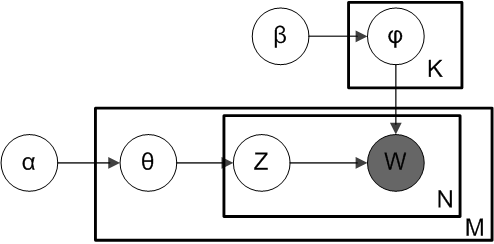
\includegraphics[scale=0.5]{lda_plate}
  \caption{Plate Notation for the LDA Method~\cite{Bkkbrad2018-yt}.
    \label{fig:lda_plate}}
\end{figure}

\renewcommand{\baselinestretch}{2.0}\normalsize
In a non-plate notation form, the simplified process for generating an LDA model across \(M\) documents is as follows:

\renewcommand{\baselinestretch}{1.0}\normalsize
\(1. Choose\, N \sim Poisson(\xi)\)\\
\(2. Choose\, \theta_m \sim Dirichlet(\alpha)\)\\
\(3. For\, each\, of\, the\, N_m\, words\, w_{m,n}:\)\\
{\hspace*{15mm} \(a)\, Choose\, a\, topic\, z_{m,n} \sim Multinomial(\theta_m)  \)}\\
{\hspace*{15mm} \(b)\, Choose\, a\, word\, w_{m,n} \sim Multinomial(\phi_{z_{m,n}}) \)}

\renewcommand{\baselinestretch}{2.0}\normalsize
Where $\underline{W}$ vectors denoting the set of $N$ words across $M$ documents, $\underline{Z}$, is the topic assignment for a word in a document, $\underline{\theta}$, is the topic distributions of each document, and $\underline{\phi}$ is the set of word distributions for each topic.

\renewcommand{\baselinestretch}{1.0}\normalsize
The total probability of an LDA model is defined as:
\[
  P(\underline{W},\underline{Z},\underline{\theta},\underline{\phi}|\alpha,\beta) = \prod^{K}_{i=1} P(\phi_i|\beta) \prod^{M}_{j=1} P(\theta_j|\alpha)\prod^{N}_{t=1} P(Z_{j,t} | \theta_j)P(W_{j,t} | \phi_{z_{j,t}})
\]
\renewcommand{\baselinestretch}{2.0}\normalsize

In LDA, the lengths of documents are said to be Poisson distributed, and that the set of probabilities  generated for each word \(w_n\) is a random multinomial dirichlet distribution. There is little reasoning for these assumptions. The use of Poisson distributions in literature seems to be a standard distribution for estimating document lengths. However, given that the lengths of documents are known parameters, the first step in the process is redundant leaving only steps 2 and 3 of the original process.

The versatility of LDA is one of its strongest characteristics. The method has seen use in a range of different settings, from filtering web spam, to the semantic annotation of satellite images. As a bayesian statistical process, it is possible to utilise other methods with relative ease given its modular nature.

In web spam filtering, LDA has been combined with tf-idf and expanded to take into consideration links that exist between documents. For spam classification, the use of LDA as a bayesian network performed worse than baseline machine learning methods, however improvements were seen when the method was expanded and combined with other statistical techniques.~\cite{Biro2008-ld}

For automatic image annotation, additional machine learning and computer vision methods can be applied to images in order transform images into collections of image features. Topics derived from a corpus of these images can be used to annotate new images introduced. Attempts at using LDA in image annotation have seen some success, whilst not all annotations from topics were correct, they were often at least conceptually related.~\cite{Feng2010-dp, Zhang2011-dn}

LDA doesn’t relate words semantically. The meanings of words in a topic are not necessarily related in any way, which is demonstrated in studies using LDA to annotate images. This means that derived topics might not provide any meaningful grouping of words. The intuition is that words in books and documents about a specific subject will somewhat relate to other words in the document. LDA might not produce thematically related topics if the documents used to derive topic distributions are varied in content. For this investigation, the potential for thematically unrelated topics is potentially a major drawback. Entities within narratives might be present throughout a whole series of books. Meaning that they may be associated with a wide range of topics. It is unclear at this stage what effect this may have on the quality of derived topics. It might be necessary to regard the same entity across two books to actually be distinct.

As a bag of words method, each unigram is treated as being unrelated to other words. Which is not true in the case of written narratives. Much of the meaning of words and relations between words are lost when used in ‘bag of word’ models. The drawback for this study is that relations between terms and entities are required. If topics were directly derived from the documents which entities were extracted from, then there would be no meaningful way of identifying how these topics apply to entities.

\subsection{Existing Implementations}

LDA is a specialised method of analysis, with only a limited number existing implementations ready and available. The popular python scientific computing library scikit-learn contains an implementation based on open source development coming from Princeton.~\cite{scikit-learn, Hoffman_undated-nx}. Genism is an alternative python library that focuses only on topic modelling methods, it is quite comprehensive in the supporting tools it provides.~\cite{rehurek_lrec}

The scikit-learn implementation of LDA outputs a set of topics each consisting of a set of word-strength pairs. Figure ~\ref{fig:lda_sklearn_output} shows the general structure of output from the method, which is the set of word distributions for the set of topics $\underline\phi$. Genism provides a more elaborate interface through which the contents of the topics an other information can be retrieved. 
\begin{figure}[h!]
\[
  \underline{lda} = \{t_1 = \{(w_1 : s_{1,1}), ..., (w_j : s_{1,j})\}, ..., t_i =\{(w_1 : s_{i,1}), ..., (w_j : s_{i,j})\}\}
\]
\caption{Output format of lda implementation in scikit-learn. where \(t_i\) is the topic, \(w_j\) is the word, and \(s_{i,j}\) is the strength of ownership between the topic and the word. \label{fig:lda_sklearn_output}}
\end{figure}

A key benefit to be had from utilising Genism, is the number of options that are available with the library. As well as a base LDA model there are varying implementations that parallelise the process or utilise proposed heirarchical approaches. Scikit-learn offers a simple method that provides minimal thrills, however, the simple implementation opens it up for extensions and adaptations in ways that Genism does not.

\section{Evaluating Topic Models}
Topic models are machine representations of word groups that have been deemed to be somehow related. The challenge for evaluating topic models is that it depends on the task which they are being applied to. Directly evaluating the accuracy of topic models is tough, as an unsupervised bayesian method, the probabilities are not interpretable, they are what they are and no ground truth exist. Where produced models can be effectively evaluated is on their efficacy at some secondary task, this could be to predict or estimate topics that might be present in documents not present in the sample used to train models.


\subsection{Perplexity}
Perplexity is a commonly used metric accross topic modelling literature, and is an estimate of how well a probability distribution or probabilistic model predicts a sample. In the literature for pLSA and LDA, perplexity is one of the main metrics used to evaluate the quality of the methods.~\cite{Blei2003-dj,Hofmann1999-qb} 

Perplexity can be calculated by subsampling a corpus into training and testing sets. By using the test set as unlablled data the perplexity of a model is measured as its ability to estimate the probabilities density of the \(M\) documents in the test set.

\renewcommand{\baselinestretch}{1.0}\normalsize
For LDA, the perplexity is defined as:
\[
  perplexity(D_{test}) = exp\{-{{\sum^{M}_{d=1} log(p(w_d))}\over{\sum^{M}_{d=1} N_d}}\}
\]
\renewcommand{\baselinestretch}{2.0}\normalsize
The probability of a word \(w_d\) is seemingly glossed over in many papers, however some methods for estimating the value have been proposed. The harmonic mean is often used as an estimator due to its relative simplicity and computational efficiency, however it has been subject to criticism regarding its suitablity for these Other methods including 'left-to'right' and a chib-style estimator have been shown to be more effective estimators.~\cite{Newton1994-ws,Wallach2008-ti,Chib1995-wq,Wallach2009-ot}

The use of perplexity as a metric for evaluating topic models does not necessarily mean that the model is correct or accurate, but rather that the model is capable of predicting a sample, not that the prediction is correct. If a topic model assigned equal proabilities accross all words in a vocabulary, then the perplexity would be high, indicating that the topic model provides no insight into the relationships between documents.

\subsection{Interpretability and Coherence}
For human interpretable topic models, it is necessary that the terms within each topic be semantically related, or that it is clear why words in a topic co-exist. Whilst attempts have been made to utilise machine learning methods in the production of coherent topic models, the evaluation of them is somewhat lax. Whilst on the surface, models appear to be more coherent with the inclusion of methods like Markov Random Fields, the coherence is often done subjectively using the opinions of juman judges.~\cite{Xie2015-wv} Even though the use of human judges may be an imprecise method of evaluation, it does provide insight into the interpretability of derived models. For tools that aim to provide users with insight into large corpora of data, interpretability of the results is a key element defining the success of the tool. With low coherence of topics and thus low levels of interpretability, communicating any extracted information becomes increasingly difficult.

Assessing the interpretability and coherence of topic models has been somewhat formalised through the proposal of a ‘word intrusion’ and ‘topic intrusion’ tests. The word intrusion test assesses the coherence of a topic by introducing words that don’t belong in a topic and asking humans to identify the misplaced word. A Topic Intrusion test is performed by introducing an incorrect topic and asking humans to identify the misplaced topic. It was found that in cases where topics are incoherent or difficult to interpret, that humans would tend to choose a word seemingly at random.~\cite{Chang2009-jr}. This method has been extended by asking humans to select two intruder words, where only one of them is actually an intrusion. The idea is that in well defined topics not only will the correct intruding word be selected, but also there will be no means for individuals to distinguish between the strength of belonging for the remaining words. If participants can't decide on what is an intruding word, then there should be a seemingly randomised selection.~\cite{Morstatter2016-co} Both approaches result in different assessments of any derived topics, there is no indication however as to which metric is a better estimate of the coherence of topics.

The precision metrics defined for word and topic intrusion tests may be of value when evaluating the quality of derived Entity Models, though they rely heavily on human evaluation of topics. Use of judges is time consuming and potentially unreliable. A more formal method of evaluating coherence was proposed by comparing word vectors formed in a semantic space built from wikipedia articles. By considering the distributional similarity of word vectors formed by pairs of words in topics, the semantic cohesion of topics can be estimated using one of a few different metrics. When considering the inter-rater agreement between the calculations and human raters, the spearmann rank correllation values had an average of  \(\bar{x}=0.77\) and a standard deviation of\(,\sigma=0.04\). The relative aggreement between each method of evaluation suggests that any of them could serve as valuable means of evaluating the coherence of topics. ~\cite{Aletras2013-oo}

Given a topic \(T = {w_1,...,w_n}\), the coherence of that topic is defined as the mean similarity of each possible word pairing \(Sim(w_i, w_j)\) where \(w_i, w_j \in T\). The similarity of two words could be one of many measures, including the cosine of the word vectors, or the jaccard coefficient.~\cite{Newman2010-op}
\[
  Coherence_{sim}(T)=\frac{\underset{i+1<j<n}{\underset{1<i<n-1}{\sum}}Sim(w_i, w_j)}{{n \choose 2}}
\]
%The precision of a topic \(k\) is defined as the number of correctly identified intruding word over the total number of intruding words. 
%
%$$P_{k}^{m} = \sum_{s} \mathds{1}(i_{k,s}^{m} = \omega_{k}^{m})/S$$
\subsection{Comparing Models}
When evaluating topic models, it is often done from the perspective selecting the best topic model. This could be doen through the use of interpretability and coherence tests, or it could be done through a models performance at some secondary task.For exploratory purposes, visual means of comparison could also be used to explore the differences between models and methods.

When regarding topics as a \(k-dimensional\) model, visualising the topic space can be challenging. One approach to comparing topic models is to look at the similarities between each topic in a pair of models. In the form of a bipartite graph, it is clear which topics in two models are conceptually similar. The bipartite graph in Figure~\ref{fig:topic_modelling_comparisons} shows that even though two methods do have different conceptual topics, there are some topics in both that are somewhat similar. The similarities and differences between the two models are seen further if relationships between documents are plotted.The noticable difference between the two topic modelling methods made visiable in the visualisation is that LDA appears to form relations between the document clusters that LSA kept distinct.~\cite{Crossno2011-sn}

\begin{figure}
  \vspace{0.3cm}
  \centering
    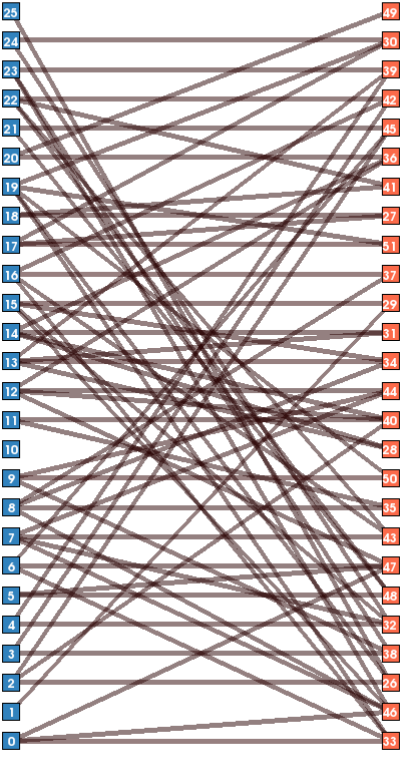
\includegraphics[scale=0.35]{lda_lsa_topic_view}
\caption{Bipartite topic conceptual similarity graph. (Middle, Right)  \label{fig:topic_modelling_comparisons}}
\end{figure}


Visualisations might be effective at explaining why a perticular model performs in a certain way at some secondary task, or it might be useful for identifying traits of models that ar valuable for perticular tasks. However, the visualisations don't provide any quantitative insight into how one model may perform when compared to another. The mapping of document relationships seen in Figure~\ref{fig:lsa_lda_compare} also suggest that further classifications can be performed on the documents, whilst LDA provides more interconnections between clusters, there are still clusters which can be used to perhaps classify future documents.

\begin{figure}
  \centering
  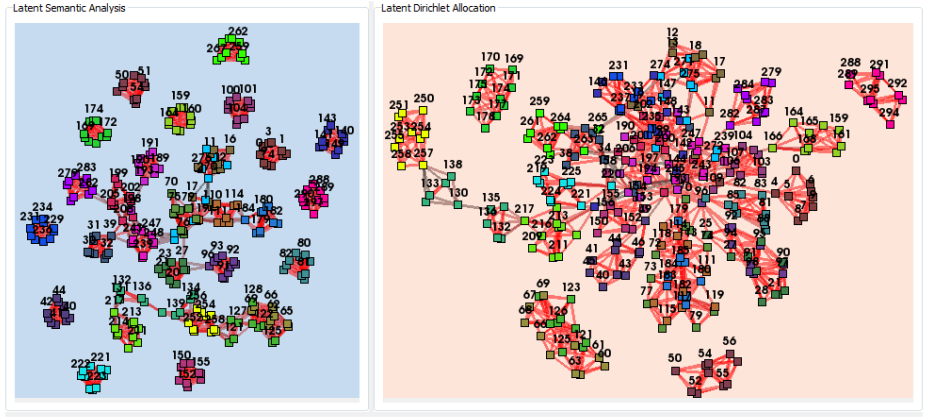
\includegraphics[scale=0.45]{lda_lsa_document_view}
  \caption{Document relationships formed by LSA and LDA topic modelling methods\label{fig:lsa_lda_compare}}
\end{figure}

\section{Entity Topic Modeling}
Entity Modelling exists as a small field of study aside from topic modelling and could be regarded as an extention of the NER domain. It relates to the extraction of entity description s, as well as the linking of distinct entities. Many of the challenges in this field stem from the high levels of ambiguity present in natural language. Attempts have been made to utilise Topic Models in the task of entitty resolution as well as forming links and relationships between entities within a document, Whilst semantic resources have been investigated as tools for the automatic tagging of extracted entities.

Entity Topic Modelling is often considered for the purpose of Entity linking, which is the task identifying how entities in a corpus relate to each other, It involves the resolution of entity mentions that refer to the same entity in order to perform optimally.

Topic models have been utilised in the task of entity linking through the application and development of specialised Entity-Topic Models.One such investigation involved finding mentions of concrete entities, such as \('iPod',\, 'Steve Jobs',\) and \(iPhone\) and forming a unifying \('Apple\, Inc'\) topic.~\cite{Han2012-gy} The approach added an additional step to the generative LDA algorithm which sampled topic, and entity assignments for each entity. The focus of the paper utilising the topical context within which each entity was mentioned, to try and resolve entities with multiple mentions through relationships that may form between entities in the model.

The Entity-Topic Models suggested are statistically sound, and perform well in predictive tasks oriented around wikipedia information. The key drawback for this study is the use of short documents to train, test, and evaluate derived models. Models were trained dataset of news articles from the TAC 2009 dataset ~\cite{Macnamee-pd}, which being short in length often benefit the assumption made in the study regarding how entities relate to the topics within the document. For longer texts and perticularly narratives, this assumption is not necessarily valid; wide ranges of topics may be present, with entities only being expressed in the context of some of these topics. The limitation of this entity-topic modelling method could come from the base LDA method. As a bag-of-words approach, 


%
%
% Chapter 3 - New Ideas
%
%
\chapter{New Ideas}
\section{Introduction}
Many different methods of analysis and topic modelling have been considered, with only those specifically discussing the generation of entity-topic models beginning to progress towards meeting the aims that this project has. Of any methods considered, each Entity-Topic Modelling approach had underlying assumptions that rendered them ineffective unless utlised under specific conditions. Additionally, no method directly addressed a need for, or the concept of, a Latent Entity.

The primary contribution of this investigation is a pipeline through which Latent Entity models can be explored. Conceptually, Latent Entity models provide a novel means of summarising, relating, and understanding written narratives. The pipeline propsed utilises a combination of new and existing approaches, with the Latent Entities being extracted using simple clustering methods. As an abstraction of underlying layers of entity topic models, it is necessary to ensure that assumptions made in literature are addressed, else flaws in any developed system ma be further apmplified.

In order to address a fundamental flaw in many aspects of literature on Entity topic models, this investigations proposes the use of a association weighting metric that allows entities to have associations with terms in a document quantified. The Gaussian Entity-Term Matrix outlined in this chapter allows the assumption that entities in a document are equally associated to terms and topics in the same document to be removed.

Evaluating topic modelling methods is a process that requires careful and considerate attention. It has been shown to be possible to evaluate topic models from a variety of perspectives, including the ability to reduce perplexity, as well as their interpretability. As an abstraction from Entity Topic-Models, typical methods for evaluation may not be applicable, alternatives are proposed in this chapter.

It becomes increasingly difficult to visualise and interpret statistical models as their complexity increases, with the meaning of models becoming obsfucated by the variability of data being analysed. Topic models are no exception to the effect that variability has on levels of obsfucation, and as methods increase in complexity, the need for exploratory tools also increases. In addition proposing a pipeline for extracting latent entities, a system for the visualisation and comparison of topic models is proposed.

\section{Gaussian Entity-Term Matrix}

The Gaussian Entity-term matrix (GETM) is a means of segmenting a given document into entities and associated terms. The matrix for a given document consists of strengths of associactions between a entity-word pairing. It functions under an assumption that the more seperation there is between two words in a document, the weaker the association is between those two  words. By modelling documents not as a bag of words, but as sequences it is possible to capture some of the relationships between different words prior to applying additional statistical methods.

Given a set of entities \(\underline{E} = \{\underline{e}_0, ..., \underline{e}_i\}\) where \(\underline{e}_i = \{e_{i,0}, ..., e_{i,m}\}\), and a set of words \(\underline{W}=\{\underline{w}_0, ..., \underline{w}_j\}\), then a matrix \(D\) when indexed by \(i,j\) can be defined as:
\[
  D_{i,j}= \sum^{|\underline{e}_i|}_{m=0}\sum^{|\underline{w}_j|}_{n=0}\sqrt{a\over{\pi}}\cdot e^{-a\cdot(e_{i,m} - w_{j,n})}
\]
\[
  D =
  \bordermatrix{&&e_0 && e_1 &&\hdots && e_i\cr
    w_0 && D_{0,0} && D_{0,1} && \hdots && D_{0,i}\cr
    w_1 && D_{1,0} && D_{1,1} && \hdots && D_{1,i}\cr
    \vdots && \vdots && \vdots && \ddots && \vdots\cr
    w_j && D_{j,0} && D_{j,1} && \hdots && D_{j,i}
  }
\]

This method makes use of the assumption that the more distance there is between two words, or the more words there are seperating two words, the less associated the two words are with each other. There are benefits and downsides to this simplification of the structure of written language. One down side to the assumption made is that, as associations between terms might exactly follow a gaussian distribution, it is possible that the associations between some terms may be exagerated, whilst others are understated. Additionally, the additive approach to handling terms occuring multple times means that there is potentially a need to normalise strengths off associations, this results in additional processing steps that could mitigated by considering alternative methods of handling multiple occurences.


\begin{table}[h!]
  \centering
    \begin{tabular}{c | c c c c}
     &Harry&Hermione&Ron&neville\\
      \hline
      loud    & 0.6 & 0.5  & 0.4  & \\
      white   & 0.1 & 0.2  & 0.1  & \\
      shock   & 0.1 & 0.2  & 0.2  & \\
      yell    & 0.2 & 0.1  & 0.3  & \\  
    \end{tabular}
  \begin{displayquote}
 ``Someone standing outside the Great Hall might well have thought some
sort of explosion had taken place, so loud was the noise that erupted
from the Gryffindor table. Harry, Ron, and Hermione stood up to yell and
cheer as Neville, white with shock, disappeared under a pile of people
hugging him.'' -- J. K. Rowling
    \end{displayquote}
  \caption{ Example GETM for entities within text \label{fig:getm_example}}
\end{table}

As Figure ~\ref{fig:getm_example} demonstrates, there results in associations between terms that are not necessarily meaningful, the association of Harry to other associations of Harry is not of value, similarly, the association of Harry to words such like 'as' and 'on' is also misleading. As the GETM is only preserving the notion of words having previously held structure and meaning, it is possible to remove perticular parts of speech that don't provide useful insights into the relationships entities have with words. Removing an entity's association to itself is not so straight forward, it requires resolving which mentions refer to which entities, and in cases where entities are either refered to by different names, or two entities share the same name, that is a difficult task. One solution is to ignore entity-entity associations in the GETM, this is perhaps the best approach given the purpose of the GETM. By removing entity-entity associations from the GETM, latent entity models will describe classess of entities, and are less likely to orient themselves around the relationships between entities.

By modelling associations using a Gaussian prior, it is then possible to adjust the hyperparameter \(\alpha\) to increase or decrease the rate at which strengths of association decline as the number of seperating words increase.

It is also possible to remove the gaussian aspect of a GETM, instead utilising different weighting functions. In some texts it might be known that words surrounding entities are associated with strengths following different distributions, thus it is possible to substitute the Gaussian for a more representative prior. 

\subsection{GETM Evaluation}
There is no need for hand crafted methods of evaluating the performance of a GETM, or the effect that a GETM has on the ability for meaningful latent entities to be derived. By fixing all values of the GETM to 1.0 (using a fixed weighting function), an entity can be associated with each term in a given document, this would encode the assumptions made in literature directly into the GETM. The fixed GETM can then be used as a baseline to compare different GETMs, whether that be adjusting parameters in the function, or utilising alternative weighting function.

As a result of GETMs being specifically formed for the task of Latent Entity extraction, it is necessary to evaluate from that perspective, the suitability of the method to other tasks would require more generalised evaluation methods. With the availability of a fixed weighting function when calculating the GETM allows for the comparion of quality between calculated Topic moels and Latent Entities with and without the use of a GETM.

\section{Entity Topic Model}
By using a GETM prior to deriving topic models words are already associated with entities, this makes extending LDA topic models a more simple task. As LDA is a bag-of-words method, each entity and its associated terms within the GETM could be regarded as a distinct document. Using GETMs add an additional set of pre-processing steps to the standard LDA algorithm.

The proportional topic distributions in an Entity Topic Model using the GETM can be calulated by multiplying the strength of association between an entity and a given word, with the word-topic probabilities calculated in an LDA model.
\[
  T_{k,e} = \sum^w \phi_{k,w} \cdot D_{e,w}
\]

Where  \(T_{k,e}\) is the Entity Topic for topic \(k\) and entity \(e\), \(D_{e,w}\) is the strength of assocation between entity \(e\) and word \(w\), and \(\phi_{k,w}\) is the topic-word probability for topic \(k\) and word \(w\).

You may wish to each topic score in an entity topic, bringing values into the \([0,1]\) range. In which case the value for each \(T_{k,e}\) where \(\underline{T}_e\) is the set of topics for entity \(e\), becomes:
\[
  T_{k,e} = \frac{\sum^w {(\phi_{k,w} \cdot D_{e,w})} - max(\underline{T}_e)}{ max(\underline{T}_e) - min(\underline{T}_e)}
\]

\subsection{Evaluating ETMs}
The evaluation of ETMs can be carried out in a similar means to many topic modelling methods, by considering the reduction of perplexity, or through determining ease of interpretation. The method proposed for calculating ETMs can also give insight into the quality of GETM as an approach.

For this thesis, ETMs are used as a means of obtaining Latent Entities, and should be evaluated from that perspective. 

\section{Latent Entities}
A Latent Entity is an abstract statistical model that approximately describes some entities within a corpus. Identifying Latent Entities is possible though clustering entity topic models extracted from a corpus. In the case of k-means clustering, each entity in a GETM matrix is expressed as distributions of entity topics and turned into an Entity-Topic Model. Each Entity-Topic Model can then be clustered in n-dimentional space on topic distributions. The center of each cluster extracted through k-means can then be labelled as a latent entity which abstractly represents entities within that cluster.

As each latent entity remains a probability distribution of entity topics, it is possible to state how similar a given entity is to a latent entity. Each similarity metric of entity to latent entity can then be used to express the entity in terms of similarities to latent entities.

\begin{table}[h!]
  \centering
  \begin{tabular}{*2c}
      \multicolumn{2}{c}{Harry}\\
      Term&Strength\\
      \hline
      Scar&0.1\\
      Magic&0.09\\
      Muggles&0.09\\
      Expelliarmus&0.05
    \end{tabular}              
    \begin{tabular}{*2c}
      \multicolumn{2}{c}{Hermione}\\
      Term&Strength\\
      \hline
      Magic&0.11\\
      Wand&0.09\\
      Superiority&0.04\\
      Unkempt&0.04      
    \end{tabular}
    \begin{tabular}{*2c}
      \multicolumn{2}{c}{Ron}\\
      Term&Strength\\
      \hline
      Drooble&0.07\\
      Magic&0.06\\
      Snigger&0.05\\
      Sherbert&0.03
    \end{tabular}
  \caption{Example entity-term associations between three entities\label{fig:example_entity_term_associations}}
\end{table}

\begin{table}
  \centering
    \begin{tabular}{*4c}
      Topics&Harry&Hermione&Ron\\
      \hline
      Topic 1 & 0.6 & 0.5  & 0.4 \\
      Topic 2 & 0.1 & 0.2  & 0.1 \\
      Topic 3 & 0.1 & 0.2  & 0.2 \\
      Topic 4 & 0.2 & 0.1  & 0.3 \\  
    \end{tabular}
    \vline \,
    \begin{tabular}{*1c}
      \multicolumn{1}{c}{Latent Entity}\\
      \hline
      0.5 \\
      0.13 \\
      0.17\\
      0.2\\
      
      \end{tabular}
  \caption{Example entity-Topic distributions for entities in Table~\ref{fig:example_entity_term_associations} and the associated Latent Entity. \label{fig:example_entity_topic_distribution}}
\end{table}

Given a set of entities (like Harry, Ron, and Hermione), a Latent Entity for this set could be derived by computing the average entity topic model. Conceptually this latent entity could describe entities that can be classified as 'wizards' or 'students'. The exact interpretion of what the latent entity represents is up for debate, in a similar way to how the topic expressed in a topic model is open to interpretation.

Latent Entities in this form could even be used as a means of assisting in the interpretation of large groups of entity topic models. A summary of ETM clusters can be given allowing for higher level overviews of latent structures within a corpus, or elements of a corpus.

\subsection{Application of K-Means}
K-Means clustering is just one approach that can be taken with regards to extracting latent entities from a collection of entity topic models. It is entirely appropriate to utilise other clustering methods, including techniques such as Fuzzy C-Means, Gaussian Mixture Models, or heirarchical style clustering. K-Means as a simple method provides a straightforward approach to finding Latent Entities.

K-Means is a method for minimising variance between clusters and as such can be described as
\[
  \underset{S}{argmin} \sum^{k}_{i=1}\sum^{}_{x\in S_i}||x-\mu||^2
\]
Given this, the equation for determining a set of latent entities for a given collection of entity topic models involves the substitution of the equation for an entity topic model \(T_{k,e}\) into the standard formula for k-means.
\section{Evaluating Latent Entities}
The evaluation of topic models is a challenging task, many techniques commonly used are inherently flawed or difficult to carry out. Many of the flaws present in topic modelling evaluation methods may be made even more pronounced if used to evaluate Entity Topic Models, and Latent. An adaptation of the intruding word test applicable to ETMs proposed here is the intruding Entity Test. Some evaluation metrics are proposed as means of evaluating the quality of latent entities.

\subsection{Intruding Entity}
The intruding entity test involves asking human participants to identify the entity that doesn't belong in a set of entities supposedly represented by a latent entity. The set of entities can be formed by choosing some amount of entities most strongly represente by a Latent Entity, then selcting and adding to the set an entity least likely to be represented by the same latent entity.

Similarly to the intruding word test, the intruding entity test is supposed to performs as a means of evaluating the cohesiveness of the latent entity. Should the set of entities actually be made of those conceptually related, then the odd entity should be identified with a high success rate across all participants.

\begin{figure}[h!]
  \centering
  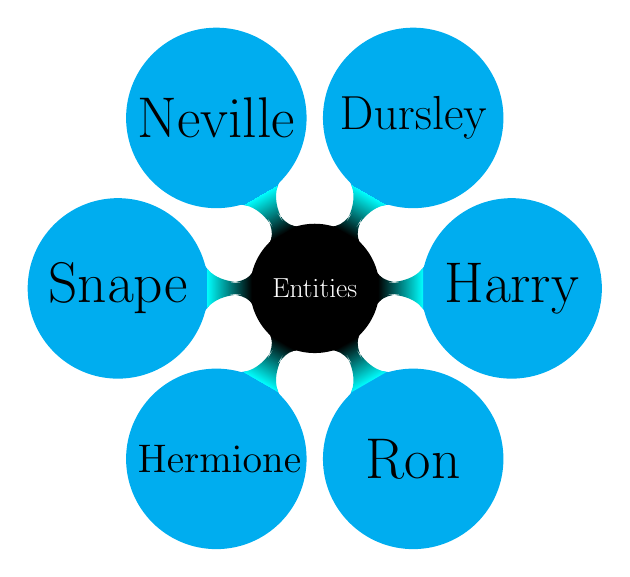
\begin{tikzpicture}
  \path[mindmap,concept color=black,text=black, scale=0.5]
    node[concept,text=white ,scale=0.4, font=\fontsize{28pt}{28pt}\selectfont] {Entities}
    [clockwise from=0]
    child[concept color=cyan] {
      node[concept,  font=\fontsize{20pt}{20pt}\selectfont]
      {Harry}
    }  
    child[concept color=cyan] {
      node[concept,font=\fontsize{20pt}{20pt}\selectfont]
      {Ron}
    }
    child[concept color=cyan] {
      node[concept, font=\fontsize{15pt}{18pt}\selectfont]
      {Hermione}
    }
    child[concept color=cyan] {
      node[concept, font=\fontsize{20pt}{20pt}\selectfont]
      {Snape}
    }
    child[concept color=cyan] {
      node[concept, font=\fontsize{20pt}{20pt}\selectfont]
      {Neville}
    }
    child[concept color=cyan] {
      node[concept, font=\fontsize{18pt}{20pt}\selectfont]
      {Dursley}
    };
  \end{tikzpicture}\\
Select the entity that does not belong the the set: \underline{\quad \quad \quad \quad \quad \quad}
  \caption{Example Set of Entities for the Intruding Entity Test.\label{fig:intruding_entity}}
\end{figure}

In Figure~\ref{fig:intruding_entity} you can see an example of how the test may look, the names of entities being presented in some format, with participants requested to select the entity that does not belong. There are a range of influencing factors that could invalidate the results of any test of this format, most notable of which is the familiarity of the participants to the reference material. In cases where individuals are unfamiliar with the narratives from which entities are drawn from, then there would be increased difficulty when selecting the conceptually unrelated entity.

Admittedly, there is a range of investigations that can be carried out to evaluate the efficacy of this method of evaluation. It might be necessary to provide participants with additional information about the set in order to allow them to make informed decisions. As the entities within the set are them selves represented by topic models, it is possible to then provide information regarding the words associated with those entities that resulted in the set of entities represented by the calculated Latent Entity.

\begin{figure}
  \centering
  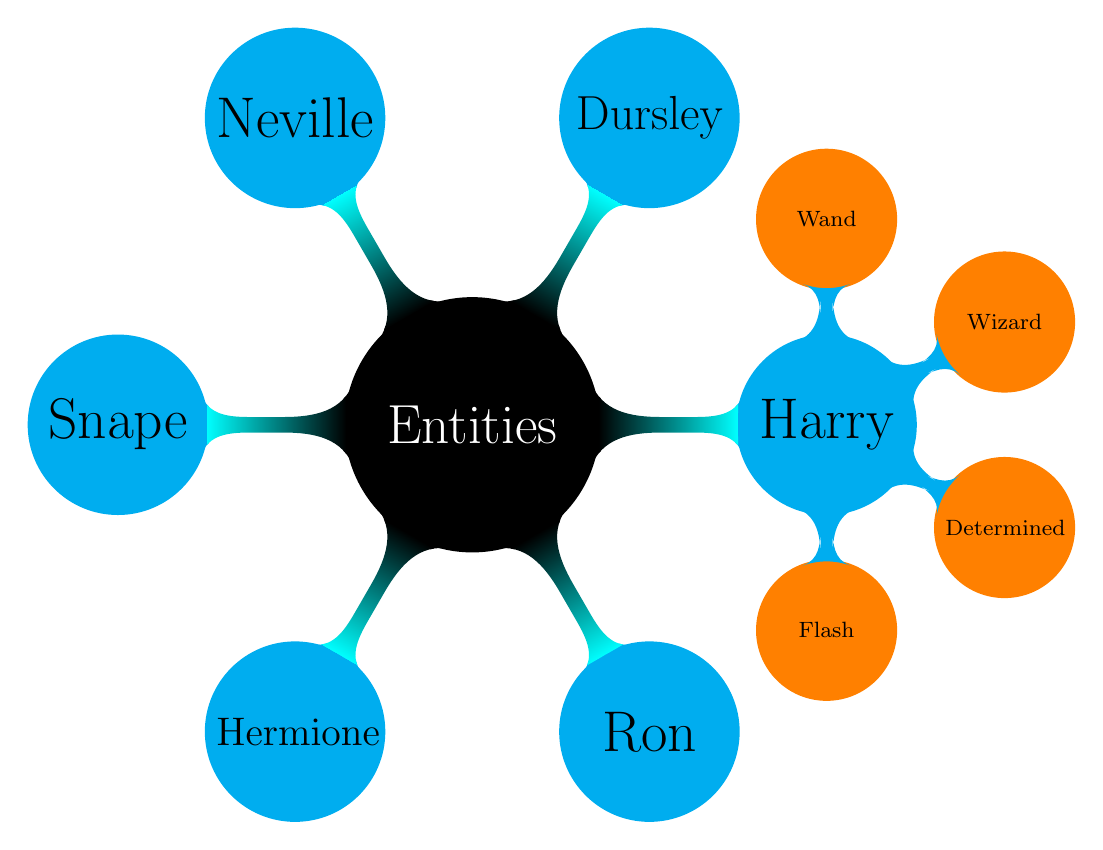
\begin{tikzpicture}
      \path[mindmap,concept color=black,text=black, scale=0.9]
    node[concept,text=white ,scale=0.8, font=\fontsize{28pt}{28pt}\selectfont] {Entities}
    [clockwise from=0]
    child[concept color=cyan] {
      node[concept,  font=\fontsize{20pt}{20pt}\selectfont]
      {Harry}
      [clockwise from=90]
      child { node[concept, color=orange, text=black] {Wand} }
      child { node[concept, color=orange, text=black] {Wizard} }
      child { node[concept, color=orange, text=black] {Determined} }
      child { node[concept, color=orange, text=black] {Flash} }
    }  
    child[concept color=cyan] {
      node[concept,font=\fontsize{20pt}{20pt}\selectfont]
      {Ron}
    }
    child[concept color=cyan] {
      node[concept, font=\fontsize{15pt}{18pt}\selectfont]
      {Hermione}
    }
    child[concept color=cyan] {
      node[concept, font=\fontsize{20pt}{20pt}\selectfont]
      {Snape}
    }
    child[concept color=cyan] {
      node[concept, font=\fontsize{20pt}{20pt}\selectfont]
      {Neville}
    }
    child[concept color=cyan] {
      node[concept, font=\fontsize{18pt}{20pt}\selectfont]
      {Dursley}
    };
\end{tikzpicture}
  \caption{Example Set of Entities with Set of Associated Terms.\label{fig:intruding_entitiy_terms}}
\end{figure}

For participants that are unfamiliar with the matrial from which the entities in the set are from, presenting the terms most strongly associated with the entities might resolve the impact that this could have on their ability to select the correct entitiy. Of course, with the addition of more information the question becomes more complex to answer, there becomes more factors to consider when determining which entity is the unrelated one.


\subsection{Evaluating Consistency}
The consistency of the proposed method for calculating latent entities can be determined by comparing the results of the process for two corpora of different documents onthe same subject. The assumptions for this method of evaluation is that the contents of books on the same subject are likely to be similar, whilst this may not be true for narratives, factual books on the same subject should hold true.

The consistency check can be used to evaluate different stages of the analysis pipeline. The GETM aspect of the system is a prime candidate for this form of evaluation. Similarly, entities within the GETM should be associated with the same or synonymous terms if assumptions regarding the similarity of two copora are true.

By using copora that are known to be similar in content would remove the perhaps dangerous assumption. However, the corpora are not the same, and thus there still remains the chance that any difference in compared models would be a result of the differences in documents between each corpora.

\subsubsection{Latent Entity Consistency}
For latent entities, it is necessary to consider entities that are present in both corpora that have been clustered differently, and the number of entities absent from one or the other document.

Considering common entities, consistency is calculated using the number of consistencies or true positive (TP), and inconsistencies or false positive (FP) entity pairings within each latent entity clusters. TP is the number of entity pairings in a latent entity cluster present in both sets of latent entities, FP is the opposite of that, the number of entity pairings within clusters not the same across both sets of latent entities.

Where $N$ is the number of Latent entities clusters, and $n_i$ is the number of entities within the latent entity cluster indexed by $i$, consistency is defined as:
\[
  Consistency = \frac{TP - FP}{\sum^{N}_{i=1}{n_i\choose2}}
\]

The defined consistency metric ranges from $-1.0$ to $1.0$. Values approaching $1.0$ mean the two sets are increasingly correlated.

\begin{table}[h!]
  \centering
  \begin{tabular}{c | c | c}
    Cluster 1 & Cluster 2 & Cluster 3 \\
    \hline
    a & 1 & x \\
    b & 2 & y \\
    c & 3 & z \\
    d & 4 & w \\
  \end{tabular}
  \quad
  \begin{tabular}{c | c | c}
    Cluster 1 & Cluster 2 & Cluster 3 \\
    \hline
    a & d & x \\
    1 & 2 & b \\
    c & y & 3 \\
    2 & 4 & w \\
  \end{tabular}
  \caption{Left \& Right: Entities Within Clusters Behind Latent Entities.\label{tab:latent_entity_clusters}}
\end{table}

An example of the consistencies and inconsistencies between two sets of latent entities seen in Table~\ref{tab:latent_entity_clusters} can be seen in Table~\ref{tab:latent_entity_consistencies}. With the total number of pairings, $\sum^{N}_{i=1}{n_i\choose2} = 16$, a $TP=4$ and $FP=12$ the consistency of these two sets of latent entities is $\frac{4-12}{16} = -0.5$. A negative value implies the latent entiteis are entirely different compositions, and are very inconsistent.

\begin{table}
  \centering
  \begin{tabular}{c | c c c c}
    Constencies
    & (a, c) 
    & (1, 2) 
    & (x, w) 
    & (4, 2)
    \\
    \hline
    Inconsistencies
         & (a, 1) 
         & (a, 2) 
         & (c, 1)                      
         & (c, 2)
         \\
         & (d, 2) 
         & (d, 4) 
         & (y, 2) 
         & (y, 4)
         \\
         & (x, b) 
         & (x, 3) 
         & (w, b) 
         & (w, 3) 
  \end{tabular}
  \caption{Consistencies and Inconstencies Between Clusters Forming Latent Entities\label{tab:latent_entity_consistencies}}
\end{table}


\subsubsection{GETM Consistency}
Calculating the consistency of the GETM method requires numerically evaluating similarity of terms associated with common entities between two GETMs. Additionally, the entities not common to both need to be incorporated into the calculation.




\section{Analysis Pipeline}
The Analysis Pipeline is a series of steps necessary for the task of extracting Latent Entities from a Corpus. Each step can be viewed as a transformation which can be applied to the results of the previous step.

The pipeline is essential to the implementation of a system which can be used to extract Latent Entity information. Without consideration of what the steps would be, the value of any developed system could be severely diminished.

Starting with raw documents, the start of the process is the tokenization of each document in the corpus. The extraction of POS tag information and Entities within the corpus can be carried out in parallel, it is necessary that both tasks are performed prior to the calculation of the Gaussian Entity-Term Matrix. From the GETM, Entity-Topics and subsequently Latent Entities can be extracted.

\begin{figure}[h!]

  \centering
  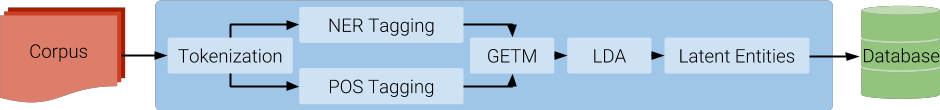
\includegraphics[scale=0.445]{pipeline_diagram_bold}
  \caption{Analysis Pipeline for the Extraction of Latent Entity Information.\label{fig:pipeline_diagram}}
\end{figure}

\section{Topic Model Explorer}

As machine representations of words most probably related topically, topic models are not always easy to interpret. Presenting only a set of terms within a topic might not provide the best insight into what that topic represents in a corpus. The challenges of interpretation are further compounded as layers of abstractions are added to a topic model. Entity Topic Models and subsequently Latent Entities would be easier to intepret when presented alongside other derived models. As such, a topic model explorer is proposed as a tool allowing the comparison and exploration of topic models, entity topic models, and latent entities.

Humans often try to understand a topic by applying a single word or small phrase as a title of any given topic. Latent Entities are abstractions of multiple Entitiy Topic Models, with each entity topic model being varying distributions of topics and words. In order to accomodate for the human need to label models, the Topic Model Explorer can accomodate for this by demonstrating how different clusters of entity topic models are similar, extracting words most siginificant across members of the cluster.

As well as allowing comparisons of entity topic models, by allowing the explorer to accomodate for the comparison of other levels of topic model extractions, it can allow individuals to evaluate the quality of each model used to describe a corpus.

\subsection{Interface}

The interface for the Topic Model Explorer is a key aspect in allowing individuals to understand the machine models extracted from a corpus. With a poor interface the system is ultimately of no use, users would struggle to use the system and thus struggle to gain an understanding of presented topic models.

The proposed structure of this interface is one that allows users to systematically progress from written text, to information about entities, and then to Latent Entity information. There is essentially four aspects of a corpus that the interface is required to demonstrate for the user to receive a complete picture of the models proposed in this thesis. Book level topic information, corpus level topic information, entity level topic information and corpus level entity topic information.

In a single narrative there can be hundreds of entities, in a large corpus the number of entities is magnitudes higher. 

\subsection{Visualisations}

\section{Project Management}
The project began with a highlevel research area, from which an iterative refinement process took place. From the idea of 'Analysing Narratives' general NLP topics were considered, with a focus on understanding the general state of the field. From looking at automatic scene generation, to understanding that even the most fundamental task of NLP (POS and NER Tagging) are still open topics of research, the project was able to focus on one active aspect of the field.

After narrowing the field down to current topics in research, the iterative process underpinned the remaining investigation and development process of the project. Agile development methodologies typically denote how small teams should conduct themselves throughout a software development life cycle, however many of the standard operating procedures of approaches like Scrum or Extreme Programming can be applied to an individual project.

\begin{figure}[h!]
  \centering
  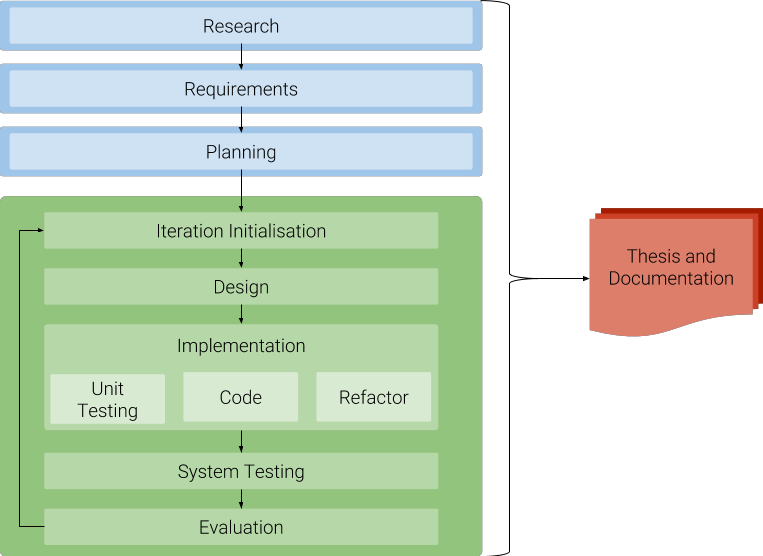
\includegraphics[scale=0.5]{pxp_process}
  \caption{Adapted PXP Process for the development of this Project and Thesis\label{fig:pxp_process}}
\end{figure}

In a form of personal autonomy, it is necessary to structure development in such a way that focus and direction is not lost, Personal Extreme Programming (PXP) is one such approach. First and foremost, PXP requires discipline and a willingness to learn and adapt, the principals of the methodology are oriented around these two points. ~\cite{Dzhurov2009-sr}

The approach can be adapted to suite a research project of this kind, where requirements and planning are bolstered with an additional 'research' process that accommodates for the investigation into research areas around the topic of the thesis. Additionally, where the methodology contains a continuous process of logging, this investigation instead substitutes logging for documenting. By documenting throughout the development process, the production of the actual thesis is a more attainable task.


\section{Professional, Social, Ethical, and Legal Issues}

With the proposal of methods and tools for the analysis and exploration of data, it is necessary to consider the professional, social, ethical, and legal issues that may be associated with the project as it comes to fruition. Ethical and legal issues are perhaps the most relevant to this project, with potential questions orienting themselves around the morality of encouraging individuals to analyse data, and copyright.

\subsection{Professional}
The development of software aiming to assist an individual in performing a task could have some unintended professional side effects. By reducing the skills required for an individual to carry out analytics task, the barriers to entering certain jobs and industries are also reduced. In critical scenarios like healthcare and security, having skilled and trained individuals is necessary to ensure that recipients of care and those under the protection of others are not harmed in any way, the reduction in workforce quality could impact businesses in this way.

An alternative view of the reduction of required entry levels to positions is that it enables others to perform better generally, either a result of more time being made available, or through the availablity of provided tools.

\subsection{Social}
The social implications of the project relate to those raised in the professional secetion. By providing means by which an individual can effectively analyse and understand a literary landscape, it allows a wider population to engage in writing with an understanding of what others enjoy and find interesting. Opening the doors to new writers of literature could bring numerous benefits to society.

The potential flaw with increasing the rate at which literature is produced is that it becomes more challenging for individuals to find literature that they want and enjoy. It potentially 

\subsection{Ethical}


\subsection{Legal}


%
%
%
%
%
\chapter{Implementation}
\section{Introduction}
For an investigation to be carried out into the possibility and efficacy of latent entities, it is necessary to begin with the implmentation of a framework through which a study can be carried out. As such implementation for this project involves the development of 3 key elements:

\renewcommand{\baselinestretch}{0.5}\normalsize
\begin{itemize}
\item Analysis Toolkit
\item Web Server Architecture
\item Latent Entity Explorer
\end{itemize}
\renewcommand{\baselinestretch}{2.0}\normalsize
The Analysis Toolkit involves the derivation and implementation of methods necessary to process and analyse corpora. Web Server Architecture involves the design and implementation of a database, Server, and API capable of allowing access to processed data and results from analysis. The Latent Entity Explorer entails the creation of a set of visualisations and tools allowing for the exploration of Entity-Topic models and Latent Entities.

Once the base framework is in place, implementation turned towards the task of evaluating the proposed process for extracting latent entities, as well as refining implementations.

\section{Architecture Overview}
The system principally follows a standard 3 layer approach to web-server architecture, requiring a database (DB), web server and API, and a client application. This implementation uses PostgreSQL as its DB of choice, as well as following RESTful practices in the API design. The web server is implemented in python, with a DB repository layer accompanying the server and API implementation. The client application (Latent Entity Explorer) is implemented using TypeScript and the Angular 5 framework.

\begin{figure}[h!]
  \centering
  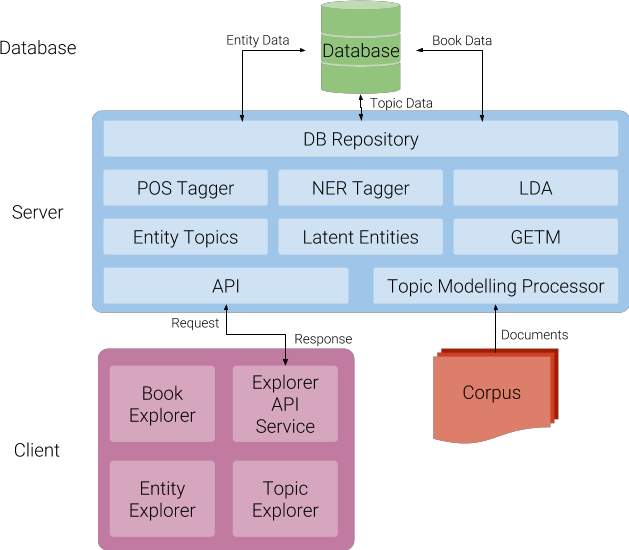
\includegraphics[scale=0.55]{architecture_diagram}
%   \begin{tikzpicture}>=latex,shorten >=2pt,shorten <=2pt,shape aspect=1

%   \matrix[matrix of nodes, row sep=5ex, column sep=1em] (mx) {
%     Database:& |[cy]| Database \\
    
%     Server:&
%     |[rs=3]|
%     \nodepart{one}DB Repository
%     \nodepart{two}Application Logic
%     \nodepart{three} REST API &
%     |[rs=3]|
%     \nodepart{one} Repository Layer
%     \nodepart{two} System Logic Layer
%     \nodepart{three} API Layer
%     \\
%     Client:& |[rs=3]|
%     \nodepart{one}DB Repository
%     \nodepart{two}Application Logic
%     \nodepart{three} REST API &
%     |[rs=3]|
%     \nodepart{one} Service Layer
%     \nodepart{two} Component Layer
%     \nodepart{three} User Interface Layer
%     \\
%   };
%   \node[ou=(mx-2-2)] (server) {};
%   \node[ou=(mx-3-2)] (client) {};
%   {[->]
%   \draw (server)edge(mx-1-2) (mx-1-2)edge(server) (client)edge(server) (server)edge(client);
%   }
% \end{tikzpicture}
  
  \caption{Architecture overview of the Latent Entity Model Analysis and Exploration System. \label{fig:architeture_overview}}
\end{figure}


Alongside the server is a set of Analysis Tools that were developed as distinct methods with utility in their own right.

\subsection{API}
The focus of the API is to allow clients to interact with data resulting from the analysis pipeline. Data to be made available will primarily consist of book meta-data, and extracted information relating to topic models, entity topic models, and Latent Entities.

Given the defined purpose of the API, and the process through which narratives can be analysed, the design of endpoints is a relatively straightforward task. The API will consist of a series of GET request endpoints for book data, as well as a small set of endpoints allowing additional narratives to be added to the system and analysed.

A Subset of the endpoints in the api for requesting data from the system can be seen in Table~\ref{tab:api_endpoints}, each of which are GET requests. There are additional endpoints that allow for other aspects of collected and extracted data to be requested, as well as POST endpoints that allow or additional documents to be added to the system.


\renewcommand{\arraystretch}{2.0}
\renewcommand{\baselinestretch}{1.0}\normalsize
\begin{table}[h!]
\centering
\begin{tabular}{r | l}
  Endpoint&URI\\
  \hline
  Book Titles        & /api/ books \\
  Book Topics        & /api/books/\guillemotleft book title\guillemotright/topics \\
  Book Entities      & /api/books/\guillemotleft book title\guillemotright/entities \\
  Book Topics terms  & /api/topics/\guillemotleft topic id\guillemotright \\
  Entity Topics      & /api/books/\guillemotleft b
                       ook title\guillemotright/entities/\guillemotleft Entity Name\guillemotright/topics \\
  Entity Topic Terms & /api/books/\guillemotleft book title\guillemotright/entities/\guillemotleft Entity Name\guillemotright/topics/\guillemotleft topic id \guillemotright \\
  Latent Entities    & /api/latent\\
  Latent Entity Topics & /api/latent/\guillemotleft Latent Entity ID\guillemotright
    \end{tabular}
  \caption{ Selection of API Endpoints. Text between guillemots represent variables of the URI.\label{tab:api_endpoints}}
\end{table}
\renewcommand{\arraystretch}{1.0}
\renewcommand{\baselinestretch}{2.0}\normalsize

From Table~\ref{tab:api_endpoints} it is clear how most of the endpoints are oriented around a book title, however, it would not make sense to follow this structure for latent entities. As latent entities are representative of a collection of entities, they are not part of any singular book, and thus are not accessed in the same means as other aspects of the API.

\subsection{Database} The database is implemented using PostgreSQL, primarily due to familiarity that is held with the DB and library interfaces for various languages (including Python and JavaScript). Additionally, PostgreSQL is an Open Source database implementation, meaning that it is a morally justifiable choice of software.

The database is a key element of the overall system, it is required to provide a persistent means of storing and accessing large amounts of data. There can be vast amounts of data extracted from a corpus, and the amount of time that a process can take to perform the task would mean days are spent waiting for a request to be completed should extracted data not be stored upon completion of analysis.

\subsubsection{DB Structure}
The Database design was to be oriented around two key concepts: Book Entities, and Topics. Building the DB around these concepts allows for some reflective structure to be maintained between the way that data is stored, and the way that users can access it through the API. The benefit to this is to a developer implementing aspects of software between the database and API, resulting in easier implementation of system logic and analysis tools that access data through the repository layer. Figure ~\ref{fig:db_erd} shows the relational structure of tables in the database.

\begin{figure}[h!]
  \centering
  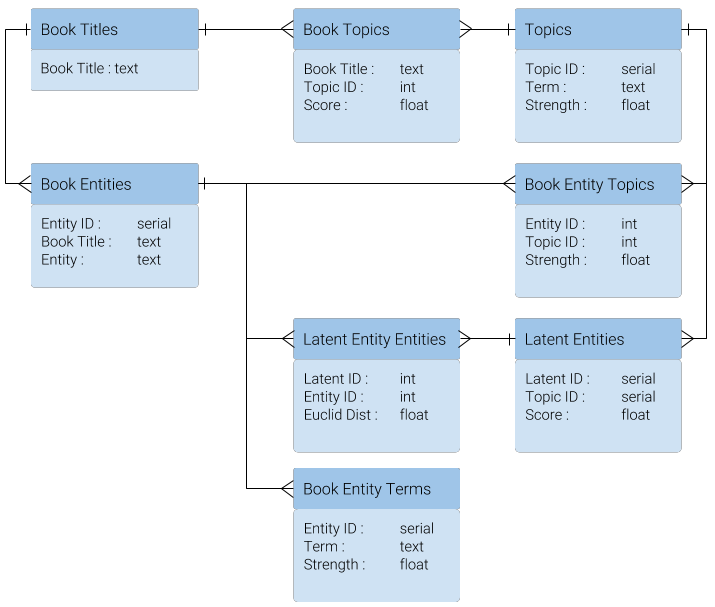
\includegraphics[scale=0.5]{db_erd}
  \caption{Entity Relationship Diagram Showing the Structure of the System's Database.\label{fig:db_erd}}
\end{figure}

A significant table to the system is the 'Book Entity Terms' table, which is a relational database form of a GETM extracted from a corpus. Principally, the table allows for the calculation of Entity Topic Models and Latent Entities to be carried out a later time, whilst also allowing an investigation into how the GETM influences resulting Models.

The tables, 'Latent Entities' and 'Latent Entity Entities' are an important pair for the system, they handle the numerical descriptions of Topics forming each Latent Entity, as well as how each entity in the corpus influenced the structure of each latent Entity.

\subsection{Server}
The Server for this system holds both the API and various distinct processing units forming the system logic. Implemented in Python, the server intergrates well with existing libraries for processing natural language and interacting with databases, it allows for the fast development of a REST API, as well as having a convenient PostgreSQL Library.

The top layer of the server, as shown in Figure~\ref{fig:architeture_overview} is the repository layer. The Repository layer handles all interactions with the database. Below the Repository layer are two layers of processing units with each providing different elements of functionality to the system, from performing POS tagging, to clustering Entity Topic Models.

Below the system logic layers sit two potential interface elements. The first, being the API allows web clients to query and interface with the system, the second is a command line interface element that allows processing of corpora to be initiated and carried out locally within the server.

\subsubsection{Repository}
Using a repository pattern approach for separating the responsibility of interfacing with the database means that a clear structure for inserting, updating, and retrieving data can be defined. In this system, the repository is utilised by both the API and the various processing units and system logic shown in Figure~\ref{fig:architeture_overview}.

The methods in the Repository are similar to the endpoints present in the API, meaning that for many of the API endpoints, there is a matching repository method for querying the DB. Table~\ref{tab:repository_methods} shows a selection of the frequently invoked methods.

\renewcommand{\arraystretch}{2.0}
\renewcommand{\baselinestretch}{1.0}\normalsize
\begin{table}[h!]
  \centering
  \begin{tabular}{>{\raggedright}p{0.34\linewidth} | p{0.63\linewidth}}
    Method & Purpose\\
    \hline
    connect\_to\_db(host, db\_name, usr\_name, pswd) & Allows for a connection to the DB to be formed using the provided user details\\
    select\_book\_titles(db) & Selects book titles from the database using a given $DB$ connection object.\\
    select\_book\_entities(db, book\_title, full\_details=false) & Selects entity names in a book specified by book title, selects entity terms if $fullDetails=true$\\
    insert\_topic\_terms(db, topic\_id, term, strength) & a Term and associated strength for a specified topic, as determined using LDA. \\
    
  \end{tabular}
  \caption{Select Methods from the DB Repository Layer. \label{tab:repository_methods}}
\end{table}
\renewcommand{\arraystretch}{1.0}
\renewcommand{\baselinestretch}{2.0}\normalsize

Aside from a single method allowing connections to the DB to be formed, the remaining methods follow a similar pattern as those specified in Table~\ref{tab:repository_methods}. As a result of the purpose of the system, as well as the design of the API, each method orients itself around Entities and Topics.

\subsubsection{System Logic Layers}
The collection of system logic layers consist primarily of methods for carrying out distinct tasks. Many of which satisfy requirements placed on the system by the proposed pipline diagrammed in Figure~\ref{fig:pipeline_diagram}.

Much of the functionality made available to the system is made available at the command line, locally on the server. This is due to the computationally intensive nature of the system, many of the tasks can take days of processing if given a large corpora. A corpus of 7 books could take approximately 3 hours to calculate a GETM for.

Each element of the System Logic Layer explored in further detail when discussing the NLP Toolkit.


\section{Corpus Pre-Processing}

Corpus Pre-Processign involves applying a set of transformations necessary to begin the analysis and creation of descriptive models. It is assumed that the corpus provided to the system will contain only the text that is to be processed. In many documents there is additional preamble, publishing information, and other elements that can be considered 'noise'. This system will not concern itself with the removal of noise within the corpus.

Tokenization is the first transformation to be applied to the corpus. NLTK provides a suite of tools capable of kickstarting any NLP project, including methods for tokenizing documents. With the option to tokenize a document into sentences, and then words, there are different approaches that can be taken to tokenization. This project uses the 'PunktSentenceTokenizer' methods of NLTK, which is an implementation of an highly effective tokenization method.\cite{Kiss2006-cm} It is important that the documents are tokenized into sentences, and then each sentence is tokenized into words, as this structure allows for more effective POS tagging.

Once each document in the corpus has sentences and words tokenized, the next stage in the processes is the application of POS tagging methods to determine the gramatical structure of each sentence. A Viterbi Decoded Hidden Markov Model (HMM) POS tagger was implemented in python, utilising the NLP tookit developed for this project. POS Tagging this document means that it is possible to apply filters to the corpus before deriving topic models from the GETM. By removing certain words tagged as certain POS (like determiners, or prepositions) it is possible to derive topics using only descriptive words, which may provide more cohesive and interpretable models.

The defined pre-processing process forms a large section of the overall pipeline, each aspect of the pipeline and preprocessing is implemented in its own distinct elements, each of which have been discussed. In order to tie each separate element into a coherent process, two scripts were developed. One to apply pre-processing at a per-document level, and one at a corpus level.

Figure~\ref{fig:document_preprocess} shows the process taken by the system to apply pre-processing methods to an individual document in the corpus. beginning with tokenization, and ending with the calculation of a GETM for that document. The process of assimilating an entire corpus of documents involves repeating the steps for including one document for a corpus provided to the document. The methods developed for the purpose of implementing this process form part of the NLP Toolkit which will be discussed in more depth.

\begin{figure}[h!]
  \centering
  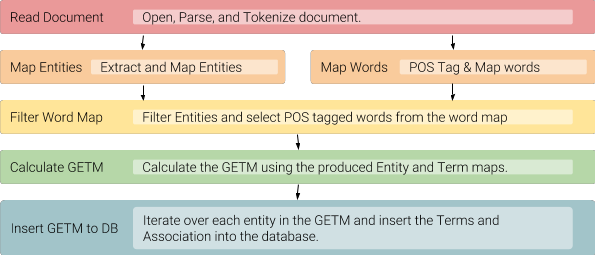
\includegraphics[scale=0.6]{per_document_process}
  \caption{Process taken to pre-process a single document in the corpus.\label{fig:document_preprocess}}
\end{figure}

\section{NLP Toolkit}
As any investigation involving the use of data in any form does, pre-processing was carried out on the collections of documents intending to be analysed. As this investigation aims to also serve as a tool from which multiple corpora can be analysed, the pre-processing steps taken need to be reproducible. The NLP Toolkit developed for this system is essentially a collection of tools that allow each document in the corpus to be pre-processed ready for the extraction of topic models and latent entities. A somewhat functional approach was used, with each method applying some transformation to a single document, or a corpus as a whole. The Analysis Pipeline defined in chapter 3 involves tasks starting with the Tokenization of plain text, and ending with the use of clustering methods to extract Latent Entities.

The toolkit can be viewed as a combination of both simple and complex NLP methods, that allow basic NLP tasks like tokenization and POS tagging to be carried out, as well as more complex GETM and topic modelling techniques.

\subsection{General NLP}
Tokenizing, POS Tagging, NER, an other pre-processing tasks are required as defined in the proposed analysis pipeline. A collection of NLP Utilities allow these tasks to be carried out within the system being developed. Table~\ref{tab:nlp_utilities} shows some of the methods developed, as well as their purpose within the system. 

\renewcommand{\arraystretch}{2.0}
\renewcommand{\baselinestretch}{1.0}\normalsize
\begin{table}[h!]
  \begin{tabular}{c | p{0.6\linewidth} }
    Method & Purpose\\
    \hline
    $sent\_tokenize(document)$ & Returns an array of string tokens representing sentences within the provided document  \\
    $word\_tokenize(sent\_tokens)$& Returns a mapping of sentence tokens to arrays of word tokens \\
    $tag\_document(word\_tokens)$ & Returns an array of POS tag sequences for each sentence of word tokens\\
    $tag\_entities(word\_tokes)$ & Returns an array of tagged entity tuples using NER tagger\\
    $cherry\_entity\_tuples(entities)$ & Returns a mapping of entity names from set of entity-type tuples\\
  \end{tabular}
  \caption{NLP Ultity Methods\label{tab:nlp_utilities}}
\end{table}
\renewcommand{\baselinestretch}{2.0}\normalsize
\renewcommand{\arraystretch}{1.0}

It is clear that some of the methods defined in Table~\ref{tab:nlp_utilities} are relatively straightforward, the method for tokenizing sentences for example, is an important yet relatively self-contained process. In contrast, the methods for applying POS tags and extracting entities  are somewhat more involved, with more going on behind the scenes.

As the process behind POS tagging is to be discussed later, The focus here is going to be on how entities are extracted. The NER tooling is not a process purpose built for this project unlike the POS tagger, the commonly used Stanford NER tagger was used to identify entities within text. As explored in Chapter 2, the difference in performance for top NER taggers are somewhat negligible. With the Stanford Tagger performing well in literature, and NLTK supporting its use in Python, it was an obvious choice of tooling.

\subsection{POS Tagging}
A Viterbi Decoded Hidden-Markov Model was implemented to perform the task of POS Tagging. The Viterbi tagger acted as a baseline from which existing taggers could be compared against. Most notably, the NLTK POS Tagger was selected as a potential POS tagging tool, this was a result of how easy the tagger is to use, and how simply it integrates with other libraries.

A dynamic programming algorithm, the Viterbi algorithm provides a comparatively computationally efficient way of decoding Markov processes, or in this case, find the most probable sequence of POS tags for a given sequence of words. This implementation followed the process described by Jurafsky~\cite{Jurafsky2014-yb}. The implemented HMM has methods for building a map of transition probabilities between states, calculating the emission probabilities for a given sequence, and calculating the starting probabilities for each possible starting state. Key methods for the tagger are outlined in Table~\ref{tab:pos_tagging_methods}.

\renewcommand{\baselinestretch}{1.0}\normalsize
\renewcommand{\arraystretch}{2.0}
\begin{table}[h!]
  \begin{tabular}{>{\raggedright}p{0.3\linewidth} | p{0.63\linewidth}}
    Method & Purpose\\
    \hline
    $calcStartStateProbs$ $(taggedCorpus, states)$& Returns a set of probabilities for the likelihood of a sequence starting with a given state, calculated from a tagged training corpus. \\
    $calcTransitionProbs$ $(taggedCorpus, states)$ & Returns a set of probabilities for the likelihood of a sequence moving from one state to another, calculated from a tagged training corpus. \\
    $calcEmssisionProbs$ $(taggedCorpus, states, obs)$ & Returns a set of probabilities for the likelihood of a given state emitting a given observation.\\
    $viterbi$ $(obs, states, startP,$ $transP, emitP)$ & Given a set of Starting, Transition and Emission probabilities, returns the most likely sequence of states for a given sequence of observations. 
  \end{tabular}
  \caption{Key methods Forming the HMM POS tagger.\label{tab:pos_tagging_methods}}
\end{table}
\renewcommand{\baselinestretch}{2.0}\normalsize
\renewcommand{\arraystretch}{1.0}

The POS Tagging model formed is essentially composed of the probabilities calculated from a corpus of pre-tagged data. It is possible to regard the methods for calculating the probabilities as being part of a training stage, where the implemented viterbi decoding is only using the model to calculate an answer. By viewing it in this way, there is potential to reduce the processing done by the system by only calculating starting state probabilities, and transition probabilities once. Unless the corpus used to train the POS tagger changes, then the probabilities behind the system won't change. The only time probabilities will need to be re-calculated, will be when determining the emission probabilities for the model. However this is really due to a flaw in the design of the tagger, instead of calculating emission probabilities for a observation sequence, the emission probabilities for all states across the whole training set could be pre-calculated.

\subsection{Gaussian Entity-Term Matrix}
At the core of the process of calculating a GETM for a document, is the weighting equation applied to determine the association between two terms in the corpus. Calculating the matrix involves going through all instances of an entity in a document, and summing the result of the weighting metric using distance between each entity instance and each term in a document.

The process requires a corpus to be separated into two sets, one set of positions for each mention of an entity, and another set for terms. The structure of data expected for the implemented is shown in Figure~\ref{fig:getm_data} methods noted in Table~\ref{tab:getm_methods} require data to be in that structure. There are additional methods allowing data to be put into this standard format.

\renewcommand{\baselinestretch}{2.0}\normalsize

\begin{table}[h!]
\centering
  \begin{tabular}{c | c}
  Entity Occurrence Set & \( \{e_0 : \{e_{0,0}, ..., e_{0,j}\}, ..., e_i : \{e_{i,0}, ..., e_{i,j}\}\}\)\\
  \hline
  Term Occurrence Set & \( \{w_0 : \{w_{0,0}, ..., w_{0,j}\}, ..., w_i : \{w_{i,0}, ..., w_{i,j}\}\}\)
  \end{tabular}
  \caption{Expected Format for Entity and Term Data for calculating GETM.\label{fig:getm_data}}
\end{table}
\renewcommand{\baselinestretch}{1.0}\normalsize



\renewcommand{\baselinestretch}{1.0}\normalsize
\renewcommand{\arraystretch}{2.0}
\begin{table}[h!]
  \begin{tabular}{ r | p{0.15\linewidth} | p{0.5\linewidth}}
  
  Method & Parameters &Purpose\\
    \hline
    Map Entity Occurrence & Entity Array & returns a python dict of entity names and associated position in a document.\\ 
    Map Word Occurrence & Document & returns a python dict of terms in a document and the associated positions in the document.\\
    Calculate GETM &Entity Map, Term Map, Weighting Function & returns a GETM object calculated from the Entity and Term maps, using the gaussian function as the default weighting function.\\
    
  \end{tabular}
  \caption{Methods used in the formatting of data and calculation of GETM.\label{tab:getm_methods}}
\end{table}
\renewcommand{\baselinestretch}{2.0}\normalsize
\renewcommand{\arraystretch}{1.0}

It is worth noting the format which the collection of entities are in once extracted from a document using the NER Tagger. Stanford's NER tagger produces an array of entities, where each entity consists of three elements, The Name of the entity in plain text, the type of entity that was extracted (person, location, or organisation), and the position of that entity in the document. 

\subsubsection{GETM Objects}
A titled-matrix class was implemented allowing matrix calculations to be performed at row or column level using column and row headings. Many of the calculations that would be performed with the GETM occur on a per-row or per-column level on values for terms and entities, and instead of keeping track of the indexes for each entity and term in the matrix this structure allows entity names and terms to be used as keys for each column and row. The ordered map and numpy matrix data structures underpin the structure of this class, with column and row keys in the ordered map linking operations to rows and columns in the matrix.

The index operator for the class allows for cells to be selected by passing either passing the index for the desired entity and term or by passing the string values of both. Additional get and set methods are implemented to accompany the index operator.

\subsubsection{GETM Visualisation}
When implementing the GETM method, a simple visualisation was implemented to allow significant terms associated with an entity to be highlighted. As the GETM was implemented in Python, Matplotlib, a python graph plotting library was used in order to make the task as straightforward as possible.

The implemented graphic is a heat map of the calculated matrix, where a coloured cell indicates the strength of association between entity and term. The darker the cell, the weaker the association. Given the number entity-term combinations occurring in a corpus, and that a GETM can be calculated for a single document at a time, the process for producing the visualisation only considered a single document at a time.

An example of the visualisation can be seen in Figure~\ref{fig:getm_visualisation}. Even on a single document, there are too many terms and entities for the visualisation to be effective, a general comparison of entities is still possible, with main characters being associated with many more terms. The implementation allows users zoom in and restrict what is shown, increasing effectiveness. Figure~\ref{fig:getm_vis_reduced} shows a closer inspection on some entities and significant terms. 

\begin{figure}[h!]
  \centering
  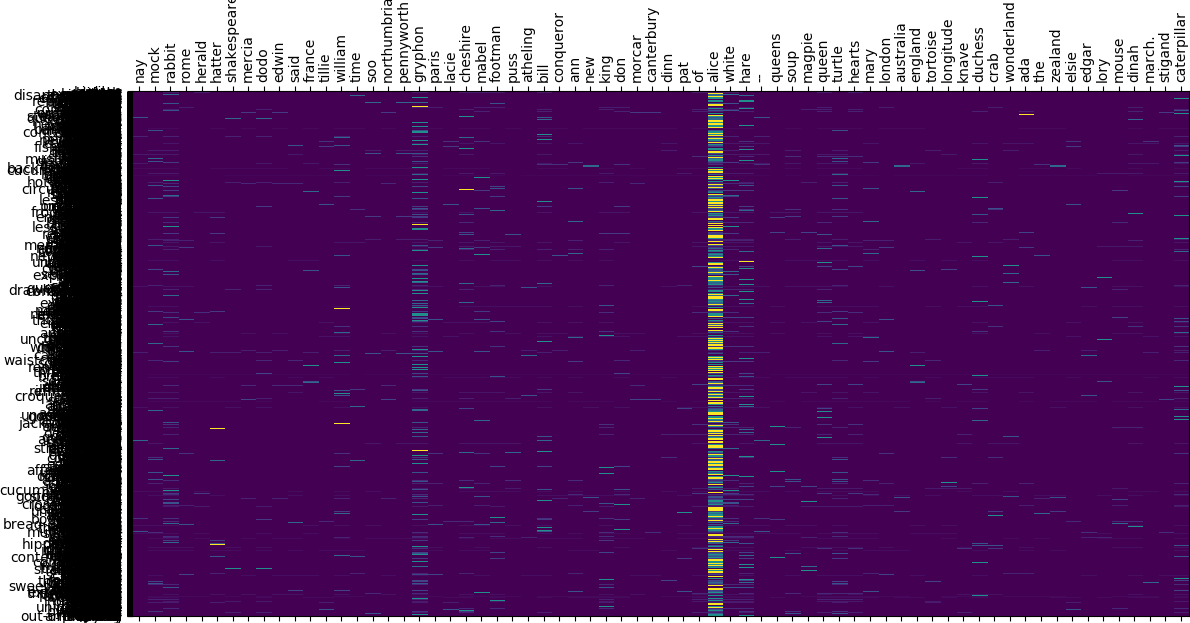
\includegraphics[scale=0.3]{getm_clutter}
  \caption{Full Zoomed-out View of the GETM Heat Map for the Alice's Adventures In Wonderland Novel.\label{fig:getm_visualisation}}
\end{figure}

\begin{figure}[h!]
  \centering
  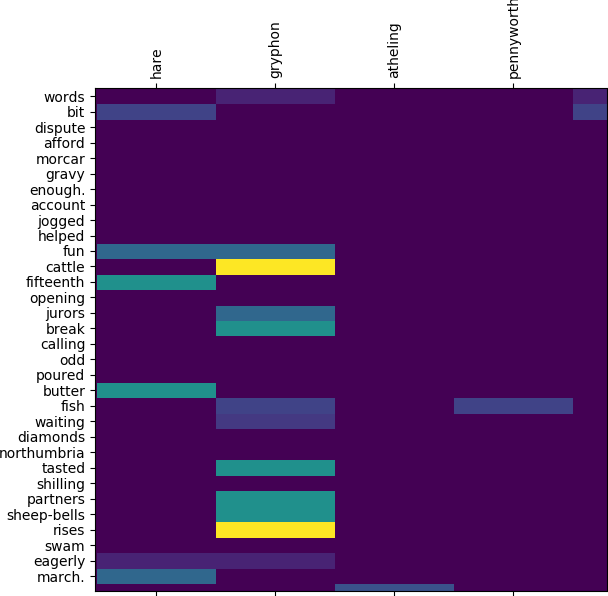
\includegraphics[scale=0.4]{getm_reduced}
  \caption{Restricted View of the GETM Visualisation for the Alice's Adventures in Wonderland Novel.\label{fig:getm_vis_reduced}}
\end{figure}


\section{Entity-Topic Model}
Entity Topic models are calculated after the calculation of the GETM. The process is similar to that of calculating topic models for a corpus of documents. Each collection of entity terms is treated as a document which is then fed into the scikit learn implemented LDA algorithm. Like other aspects of the pipeline, this element is also developed in python.

The scikit learn implementation produces word distributions for each topic, in this implementation, the resulting topics can be used to produce entity topic models by looking at the proportional distributions of terms in the GETM for an entitiy, and the score associated with that word across the topics. Topic scores for an entity are normalised in order allow consistent comparisons across entities. Large numbers of Entity Topic Models can be produced in this approach, from which Latent Entities can be calculated.



\section{Latent Entity Clustering}
Clustering was proposed as a potential means of extracting Latent Entities from a collection of Entity Topic Models, specifically the k-means method. The scikit-learn library contains a range of clustering implementations, including a simple k-means algorithm that produces a k-means classifier object. 

With Entity Topic Models stored in the system's DB, the process of calculating Latent Entities begins by querying for the model of each entity. After formatting the results of the query using the Numpy library the K-Means clustering process can take place.

The result of the clustering process is a set of center clusters, each of which represent a Latent Entity Model in a format mirroring the structure of the input. Once the Latent Entity Topic Proportions are determined through clustering, a mapping of Entity Topic Models to Latent entities can begin. The euclidean distance in Topic Space between an Entity Topic Model and Latent Entity Model indicate the degree to which an entity is represented by a Latent Entity.

Figure~\ref{fig:etm_plot} shows a scatter plots for 648 Entity Topic Models. When presented in this format it is somewhat visibile that there are some potential clusters or underlying structures. Significant topics in this form for entities extracted from 3 narratives are Topics 3, 4, and 8.

With only 3 narratives there is the potential for the diversity of topics derived from the GETM to be too low to be of practical use, the lack of diversity manifests itself in the similarity of each Entity Topic Model in Topics 0, 1, 2, 5, 6, 7, and 9. An alternative intepretation is that there is going to be some degree of similarity between entities, and there could concievebly be a minumim set of similarities that exist between all entities in a corpus. The consequences of this in the implementation is seen when selecting numbers of Latent Entities as well as the number of topics to calculate in other stages.    

\begin{figure}[h!]
  \centering
  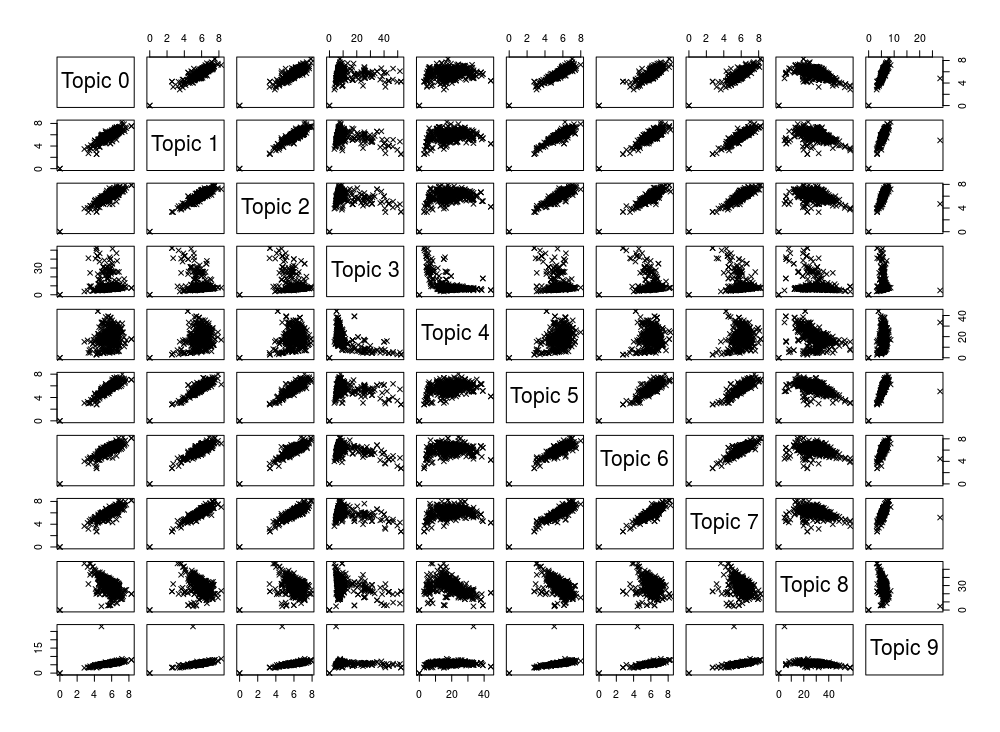
\includegraphics[scale=0.55]{entity_topic_models}
  \caption{Pairwise Matrix of Scatter Plots for Topic of a Collection of Entity Topic Models.\label{fig:etm_plot}}
\end{figure}

\section{Latent Entity Explorer}
The interface for the exploring Latent Entities was designed from a personal perspective as a result of its use in supporting the development of other aspects of the system. Implemented using TypeScript and the Angular 5 web framework, the application allows for system to be designed in terms of components, which correspond effectively to the stages seen during the development of the analysis pipeline.

The implemented structure of the application can be seen in Figure~\ref{fig:web_app_structure}, the application interacts with the server entirely through a simple Angular 5 service. The Explorer API Service is essentially a singleton class which each other component has access to, it makes available methods necessary for issuing requests and receiving responses and does so using an Observer/Subscriber approach. 

There are 4 main components for the application, three of which are controllers involved in allowing users to explore books, topics, and entities. The fourth Controller is a higher level component that co-ordinates across all elements of the application. In addition to each controller is an equivalent view that allows the user to interact with that aspect of the system. The Explorer View is composed of the other views of the application, when users interact with UI elements, it is through the Explorer View.

\begin{figure}[h!]
  \centering
  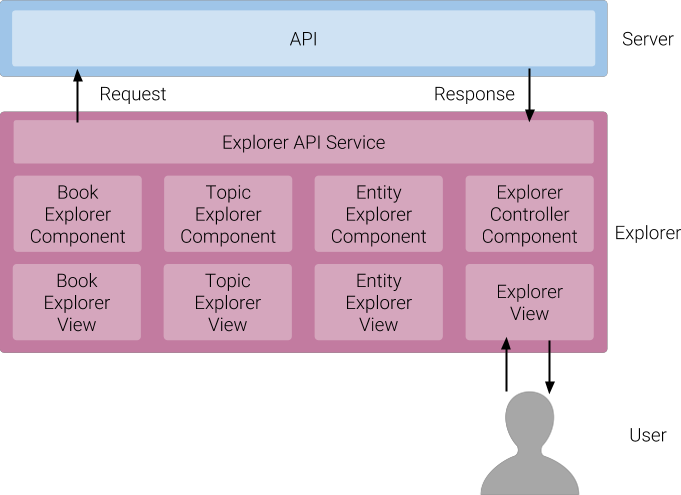
\includegraphics[scale=0.65]{web_app_structure}

  \caption{Structure of the Web Application. \label{fig:web_app_structure}}
\end{figure}

\subsection{UI and Navigation Design }
In order to provide a succinct and mobile friendly interface, each element of the system is thought of in terms of components and panels. Each panel provides access to a distinct feature, be it a visualisation of topic distributions in the corpus, or the comparison of entity topic models. Each panel is associated with a component that acts as a controller for that UI element. Though this thesis is not a study of effective UI design, having a usable interface assists in communicating the results of analyses.

Figure~\ref{fig:ui_layout_sketchup} shows initial layout and structure intended to guide the UI of the application. Each panel is of a fixed size, and shows information about a specific aspect of the corpus. Listings of book titles, entities, and topic terms will all be held within separate components. The interface read from left to right, top to bottom, and as progressing though the application, different elements are required to be selected so that more information can be displayed.

Latent Entities are models describing the entire corpus, so wouldn't require the user to specify any information. In order to view Topic Models and information about individual entities in a book, the user would be required to first select a book, and then select an entitiy to view information about that entity.

\begin{figure}[h!]
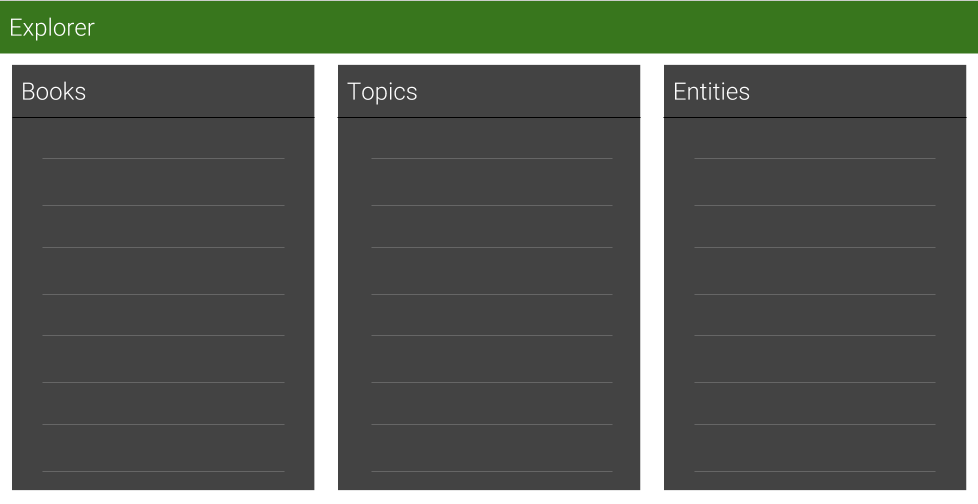
\includegraphics[scale=0.4]{ui_layout_drawing}
\caption{UI mockup layout. \label{fig:ui_layout_sketchup}}
\end{figure}

\subsection{Book Explorer}
The Book explorer provides an interface for searching and selecting books analysed in the system, so that data and extracted information resulting from the analysis pipeline can be viewed. Split into two elements, the controller for this part of the application allows users to search for books that have been analysed, as well as initiate requests for book information through the API Service when users select a book. The view elements of the Book Explorer the follows the panelled style outlined when discussing the UI and Navigation Design.

Delving into details of the corpus begins with the Book Explorer, for users to view entities and thus information about entities, they must first select a book from the listing of analysed books. Upon selection, the component emit's the book selection, which is recieved handled by the acompanying Topic and Entity Explorer components. In addition to emitting events to other component, the Book Explorer invokes method of the API Service for making requests to the server.

Visualising information at a book level is not of particular interest to this investigation, as such the only visualisations associated with each book is actually of the topic distributions and is handled in the Topic Model Explorer component. It is however through the book explorer component that user can signal to other components which entity and topic information it is they wish to view.

\begin{figure}[h!]
  \centering
  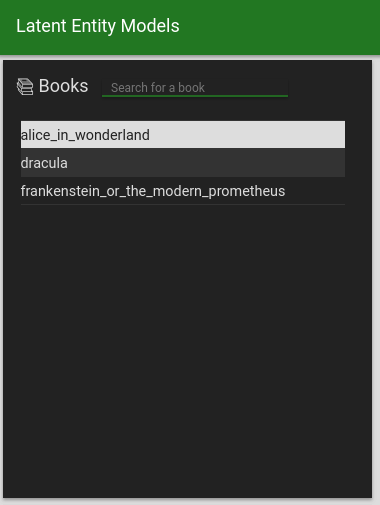
\includegraphics[scale=0.5]{book_list}
  \caption{Book Selection Component for Navigating the Explorer.\label{fig:book_selection}}
\end{figure}

Figure~\ref{fig:book_selection} shows the panel for selecting books, once the user selects a book, a collection of entities and the numerical topic distribution for the selected book is requested from the server. The search operates by making a request through the API Service for book titles containing the entered string.


\subsection{Topic Explorer}
The Topic explorer is a key component of the application as it provides book level topic information extracted from a corpus, some information about the topics extracted using LDA, as well as the topic distributions for a document selected in the book explorer. Additionally, there is an exploratory visualisation for comparing the topic distributions of each document in the corpus.

The Book-Topic Distributions are presented in the form of a stacked bar chart, where each block on the stack represents the proportion of the document that a topic represents the document. Each colour in the stack represents a different topic, with the same colour representing the same topic across each stack for each document, the panel in the application for this visualisation is shown in Figure~\ref{fig:book_topic_compare}.

\begin{figure}[h!]
  \centering
  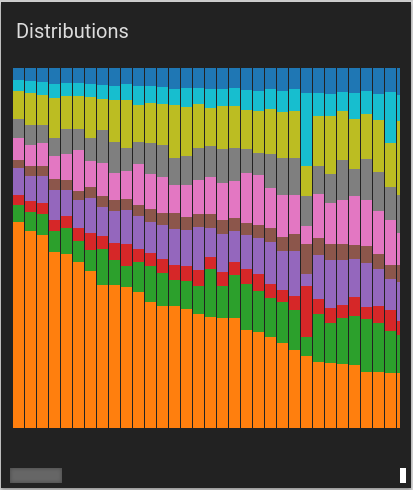
\includegraphics[scale=0.5]{topic_distr}
  \caption{Book-Topic Distribution Panel for Comparing Topical Makeup of the Corpus. \label{fig:book_topic_compare}}
\end{figure}

The construction of the chart is done dynamically, making a request for the topic distributions of analysed books in the system. For larger copora, the application would issuing requests and producing the figure for 100,000's of documents, however for this prototype and with complete control over the size of the corpus that is not an issue that would be encountered. As the visualisation is data-driven using the d3.js library, it is possible to interact and inspect elements of the figure. Users can sort the graph from highest to lowest on topic distribution. Meaning that users can see which book is most represented by each topic. Presenting topics in this way allows for quick visual comparison of documents and topics, as well as providing insight into how a documents topic structure may have an effect on the Entity Topic Models topical make up. 

When a document is selected from the Book Explorer, this component uses the emitted book title and the API Service to make a request for the numerical topic distribution of the chosen book. The percentage proportions of topics in the document are shown in a panel in a listings format, and allow individuals to compare Entity Topic proportions to the Document the entity resides in. Figure~\ref{fig:book_topic_inspect} shows what the user would be presented with.

\begin{figure}[h]
  \centering
  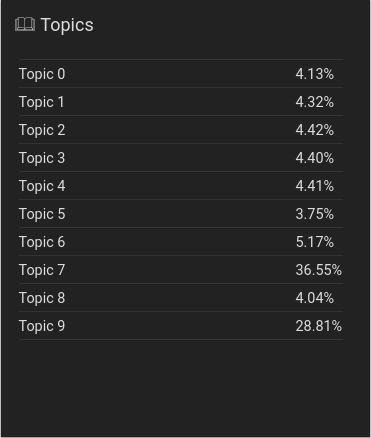
\includegraphics[scale=0.5]{book_topic_distr}
  \caption{Book-Topic distributions for a Selected Book. \label{fig:book_topic_inspect}}
\end{figure}

\subsection{Entity Explorer}
The Entity Explorer Component handles each panel associated with Entity information. Including the selection of entities for further inspection and comparison with other entities, as well as any visualisations for an entity.

When an entity is selected in the Book Explorer component, the Entity Explorer component is signalled that the user has made a request for more information, the component then makes a request through the API Service to the server, requesting entity information for the selected book. Figure~\ref{fig:entity_listing} shows a view of all entities extracted from the selected book, users can click on an entity to view the Entity Topic Model of that entity, or press the green addition box to add it to to a entity comparison panel. Similarly to the book listing panel in the Book Explorer component, users can search for entities using text to filter entities not containing the query string.

When selecting an entity to be added to the comparison view, the entity is not removed from the listing, and can still be selected for a more detailed inspection if desired. The entity cannot however, be added to the entity comparison panel if it is already present. The Entity Explorer component maintains an array of Entity JSON Objects to allow the tracking of inspected entities.
\begin{figure}[h]
  \centering
  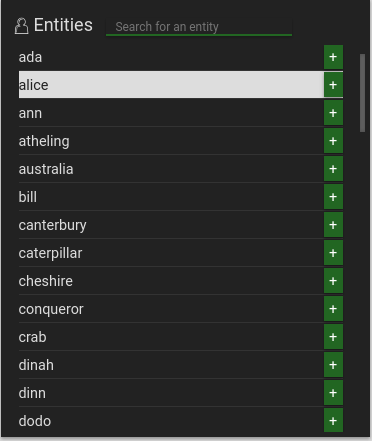
\includegraphics[scale=0.5]{entity_listing}
  \caption{Entity Listings for the Selected book (Alice's Adventures In Wonderland)\label{fig:entity_listing}}
\end{figure}

When an entity is selected for further inspection, users are presented with a breakdown of the Entity Topic model and GETM results for that entity. Figure~\ref{fig:entity_topic_pct} shows the topic distributions for the selected entity 'Alice' from Alice's Adventures Into Wonderland, the significant topics for this distribution are Topics two and seven. A visualisation of this distribution, would not be so informative given the position of the panel in relation to the other panels. Users can compare the percentage proportion of a topic in this panel to the percentage proportion of the topic in other components.

In order to provide some user insight into terms associated with an entity that contribute to an entity's topic model, a panel was formed listing the terms and their strength. Figure~\ref{fig:entity_top_terms} shows the most prominent terms for the entity 'Wonderland' in Alice's Adventers in Wonderland.  As entity terms were filtered when calculating the GETM, the term 'wonderland' associated with the Entity 'Wonderland' are not actually referring to the same thing.

\begin{figure}[h]
  \centering
  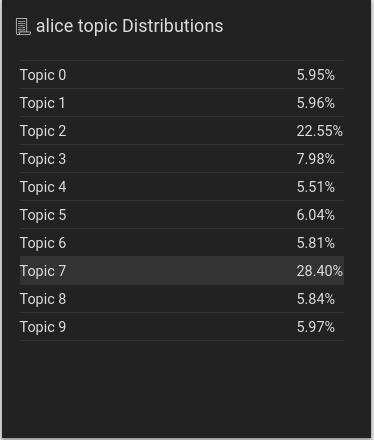
\includegraphics[scale=0.5]{topic_dist_pct}
  \caption{Entity Topic Distributions for Entity Topic Model. \label{fig:entity_topic_pct}}
\end{figure}


\begin{figure}[h]
  \centering
  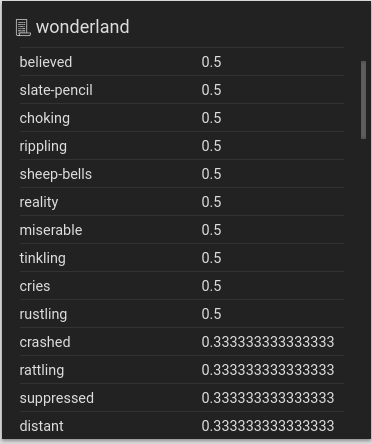
\includegraphics[scale=0.5]{entity_getm_top}
  \caption{Top Terms Associated with Entity resulting from GETM. \label{fig:entity_top_terms}}
\end{figure}

The panel for comparing entity topics is shown in figure~\ref{fig:entity_compare}, which is the primary interface through which users of the system can begin to compare the topic models that represent an entity. Where entities were added using the '+' in a green box on the entity listing panel, entities can be removed from the comparison panel by pressing the '-' in a red box.

\begin{figure}[h]
  \centering
  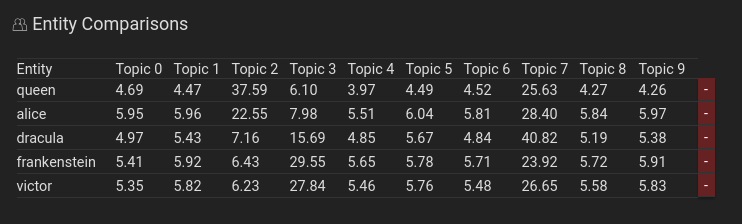
\includegraphics[scale=0.55]{entity_compare.png}
  \caption{Entity Comparison Panel for inspecting Entity Topic Distributions\label{fig:entity_compare}}
\end{figure}

%
%
% Chapter 5
%
%
\chapter{Results and Evaluation}
\section{Introduction}
This evalation the implmented system is oriented around the key features discussed in previous chapters. Numerical evaluation methods are applied to the implemented POS Tagger, GETM, and Latent Entity methods using a combination of new and some standard approaches seen in literature, whilst a qualitative assessment of the developed interface and system as a whole will be given. Additionally, an evaluation of the project from the perspective of professional, social, ethical, and legal issues outlined previously will be given. As the motivation of the study was on providing individuals with interpretable means of assessing the 'meta-data of their lives', much of the evaluation will be on the interpretability of the developed models. 


\section{Evaluation Corpora}
Before starting any evaluation involving natrual language text, it is important to consider corpora that may be suitable for use in analysis. This thesis considers a pairing of copora where one consists of a series of novels, and the other consists of summaries of the opposing novels. The same corpora will be used in the evaluation of both the GETM, and Latent Entity models. By comparing summaries of novels to the full books, there is potential for insight to be gained regarding the consistency and ability of the models when used in a document summary context. In order to comply with UK Copyright law, books could only be considered as candidates if they were legally available to the author of this thesis.

Whilst only forming a relatively small corpus, the Harry Potter series by J. K. Rowling were selected as the narratives through which the evaluation of the thesis could be carried out. This is for numerous reasons, firstly, it is known that there are characters present throughout the series, as well as some that arent. By having entites that aren't ubiquitous it is possible to gain insight into why there may be differences in any consistency tests. Another important factor in the use of these documents, is that they are familiar to the author, and thus a qualitative insight can be provided when evaluating the interpretability and cohesion of the models.

\subsection{Harry Potter Corpus Statistics}

The Harry Potter corpus contains 1,414,420 words ($\bar{x} = 202060$), with a total of 3275 entities extracted from all documements. Topic distributions of the Harry Potter novels are shown in ~\ref{tab:hp_topics}, knowing these distributions will show if there is potential for differences in entity topic models about entities common through the series. Figure~\ref{fig:hp_topics} visually shows some of the differences between the documents in the corpus.

Notably, there is only significant variance in 3 out of the ten topics accross the novels. which manifests itself through the changing distributions shown accross the stacked bar chart. whilst the other topics do see noticable changes in proportions, none are quite as significant as topics 1, 3, and 8. Which on a corpus of related documents, should not be overly suprising. For comparison, figure~\ref{fig:book_topics_large} shows topic distributions for a corpus of over 300 narratives, including the harry potter novels which are highlighted by the black rectangle. The variation between the novels is even less when viewed in the context of a wider corpus.

\renewcommand{\baselinestretch}{1.0}\normalsize
\renewcommand{\arraystretch}{1.2}
\begin{table}[h!]
  \centering
  \begin{tabular}{c || c | c | c | c | c | c | c | c | c | c }
    &     \multicolumn{10}{c}{Topic (\%)}\\
    Book                 & 0     & 1    & 2     & 3      & 4    & 5     & 6    & 7     & 8     & 9 \\
    \hline
Philosopher's Stone	&5.16&	19.62&	5.45&	22.29&	4.94&	5.09&	7.04&	5.31&	20.15&	4.96\\
Chamber of Secrets	&4.77&	19.73&	4.83&	15.51&	4.54&	4.91&	10.80&	5.02&	25.06&	4.82\\
Prisoner of Azkaban	&4.33&	33.30&	4.27&	14.21&	4.01&	4.40&	5.50&	4.22&	21.61&	4.16\\
Goblet of Fire	        &4.68&	19.82&	4.67&	16.09&	4.31&	4.69&	5.94&	4.71&	30.60&	4.48\\
Order of the Phoenix    &4.66&	25.97&	4.54&	16.07&	4.40&	4.68&	6.22&	4.72&	24.08&	4.67\\
Half-Blood Prince	&4.77&	20.05&	4.58&	17.20&	4.35&	4.69&	6.04&	4.78&	28.92&	4.62\\
    Deathly Hallows	&4.88&	18.61&	4.58&	23.68&	4.47&	4.82&	6.27&	4.80&	23.27&	4.62\\
    \hline
    $\over{x}$          &4.75&	22.44&	4.70&	17.86&	4.43&	4.75&	6.83&	4.79&	24.81&	4.62\\
    $\sigma$            &0.25&	5.37&	0.37&	3.63&	0.28&	0.22&	1.81&	0.33&	3.77&	0.25
  \end{tabular}
  \caption{Topic Distributions for the Harry Potter Novels by J. K. Rowling \label{tab:hp_topics}}
\end{table}
\renewcommand{\baselinestretch}{2.0}\normalsize
\renewcommand{\arraystretch}{1.0}

\begin{figure}[h!]
  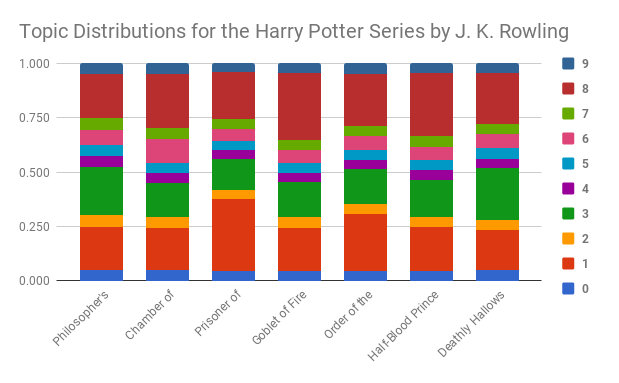
\includegraphics[scale=0.65]{hp_topics}
  \caption{Propotional Topic Distributions for the Harry Potter Novels by J. K. Rowling \label{fig:hp_topics}}
\end{figure}

One of the factors influencing the distinct similarity between narratives in the larger corpus is the inclusion of entities as terms when calculating the LDA topic models, for the reduced corpus of harry potter novels, the entities have been removed. When entities were left in as terms for calculating topics, the method distinguished between novels based on the characters, as opposed to any differences in writing style. With entities left within the calculations, Harry Potter and The Prisoner of Azkaban as well as Harry Potter and the Order of the Phoenix were indicated as being very similar documents. When inspecting the topic word distributions, the topics most strongly representing these documents were made up of terms like 'sirius' and 'black', which are referring to an entity prominent in both documents.

Without considering entities within the documents, the distributions are much more similar, however there are still differences between them. Some degree of similarity within documents is expected, given that they are from the same series, and oriented around the same sort of stories.

Key terms in the Topic-word distributions can be seen in table~\ref{tab:hp_topics_terms}, considering the terms that form the topics might provide some insight into why some documents in the corpus deemed so topically similar. However with topics-word of 1000 terms, viewing a small portion might not provide accurate insights.

\begin{table}[h!]
  \centering
  \resizebox{1.0\textwidth}{!}{%
  \begin{tabular}{c | c | c | c | c | c | c | c | c | c}
    0&	1&	2&	3&	4&	5&	6&	7&	8&	9\\
    \hline
diary&	elf&	tent&	dementors&	elf&	elf&	tent&	elf&	elf&	dementors\\
heir&	apparently&	elf&	elf&	tournament&	map&	dementors&	lesson&	task&	firebolt\\
elf&	dementors&	locket&	remained&	map&	remained&	elf&	surface&	tournament&	lesson\\
prefect&	homework&	goblins&	hastily&	task&	tent&	ought&	task&	prime&	dementor\\
attacks&	ought&	horcruxes&	apparently&	dementors&	task&	lesson&	ought&	lesson&	homework\\
clicking&	position&	ought&	triwizard&	apparently&	locket&	prime&	gazing&	apparently&	map\\
toilet&	lesson&	dementors&	highly&	ought&	ought&	task&	elves&	hastily&	gazing\\
petrified&	tone&	vault&	tent&	triwizard&	dementors&	apparently&	map&	map&	elf\\
camera&	thoughts&	apparently&	thoughts&	troll&	lesson&	locket&	dementors&	triwizard&	ought\\
wife&	ropes&	remained&	ought&	lesson&	conversation&	thoughts&	prime&	remained&	rat
  \end{tabular}}
  \caption{Top Ten Words in the Topic-Word Distributions of Calculated Topics for the Harry Potter Corpus\label{tab:hp_topics_terms}}
\end{table}

Many of the topics are actually very similar with regards to the terms which they contain. The term 'elf' is ranked within the top ten for all topics. Whilst the term 'Ought' occurs as a top ten in eight topics.  This not only highlights the significance of many of the terms, but also suggests a lack of diversity in the vocabulary for each document. Some terms however are not present through each novel, but still remain present across multiple topics, including 'triwizard' which is prominent only in 'Goblet of Fire'.

With regards to the coherence of the topics, there is little semantic relations between the terms of topics, however within the context of the novels, some relationships can be identified for example, the terms 'goblins', 'vault', 'locket', and 'horcruxes' are all related within the novels. Within the Harry Potter universe, the banking vaults are managed and guarded by goblins, whilst a significant item often simply referred to as the 'locket' was a horcrux. Additionally, a horcrux was also stored within a vault guarded by goblins. 


\clearpage

\begin{multicols}{2}
  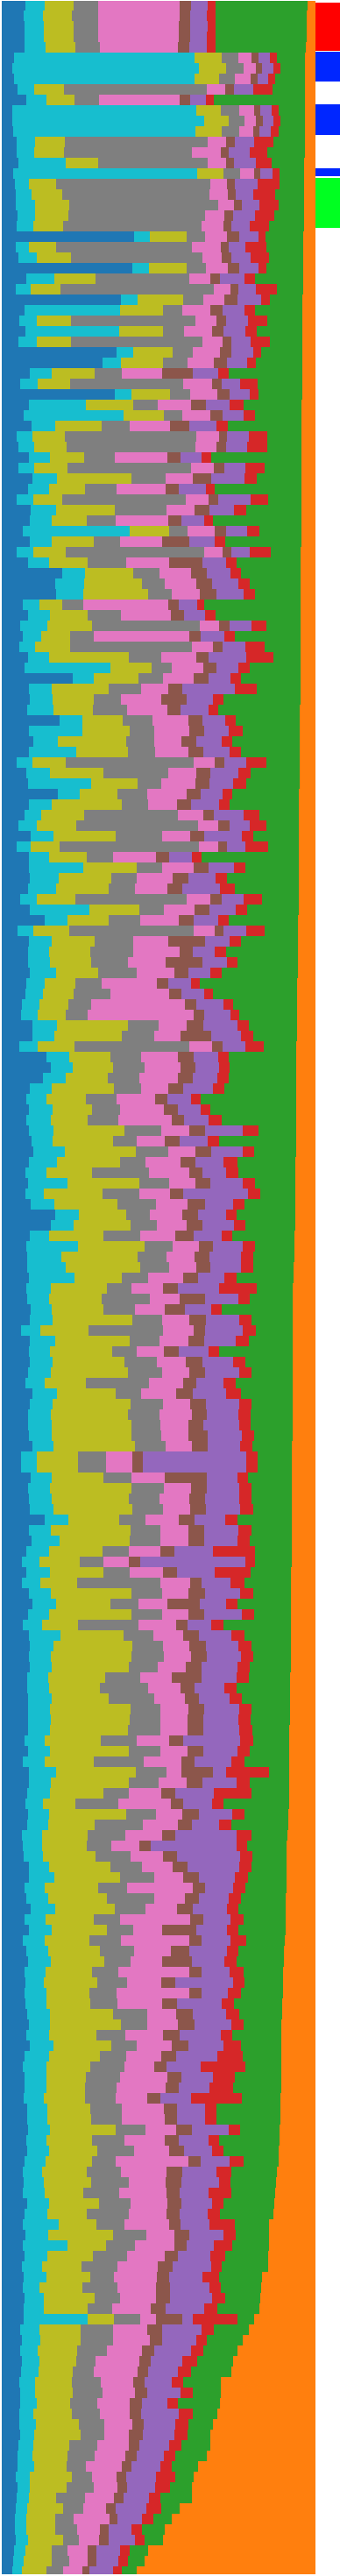
\includegraphics[ width=0.9\linewidth, height=0.9\textheight]{book_topics_large}
  \captionof{figure}{Book Topic Distributions for a Large Corpus of Fiction and Non-Fiction Books \label{fig:book_topics_large}}
  
  \columnbreak
  
  When you consider the topical structures of large corpus of documents, you can see how there are  groups of documents have distinctly similar topic distributions, perticularly when ordered by the contribution that a topic makes to a documents distributions. Three document groupings are highlighted in figure~\ref{fig:book_topics_large}, where each colour represents a topic and each line represents a document. Larger blocks of colour indicated a larger contribution that a topic has to a given document distributions.

  The set of rows indicated by the red block are books written by the author G. R. R. Martin, and include the novels behind the popular TV show 'A Game of Thrones', The the rows indicated by blue are the Harry Potter Novels that are used to evaluate other aspects of the project, the rows indicated by the green tag are narratives written by Agatha Christie.

It turns out that for this large and diverse corpus, the topics that have been extracted are oriented around narratives that exist as part of a larger series, or books that are similar in subject matter. Whilst Topics 5 (pink), 6 (grey), and 8 (cyan), are essentially topics describing books written by G. R. R. Martin, Agatha Christie, and J. K. Rowling respectively, other are strongly indicative of other author's writings.
\end{multicols}

Topic 3 (red) is a relatively small portion2 of all narratives, however the books that this topic represents the most are all novels by Dan Brown. In contrast, topic 0 (orange), which represents a large proportion of many narratives, are largely factual or phyics related documents, with the books most represented by the topic being authored by Richard Feynmann.

Whilst not the focus of this investigation, is not necessarily on the topic models of narratives, it is interesting to see how topic models can represent differences in an authors writing. It suggests that thare are distinct differences between some authors, whilst there remain major similarities between others.

One concern is that in large series of narratives entities are often present throughout each document, perhaps resulting in any given topic's word distribution consisting primarily of entities from a series. When looking closer at the terms that form the topics, there are some topics that almost entirely consist of entities, whilst others are general terms relating to a specific subject.

The top terms for topic 8 are: 'Harry', 'Ron', 'Hermione', 'Percy', and 'Annabeth'. With 'Harry' being scored as twice as representative as 'Ron', labelled as the second most prominent entity. When considering the makeup of Topic 8, it is then clear why the Harry Potter novels feature such a high proportion of the topic.

The top terms for topic 0 are: 'Energy', 'Field', 'Example', 'Species', and 'data'. When looking at these terms, it is unsuprising to see that non-fictional and scientific documents recieve a high proportion of the topic.

Agatha Christie novels are strongly represented by topic 6, the top terms of which are: 'Poirot', 'Mr', 'Miss', 'Mrs', and 'Sir'. When looking in one Agatha Christie novel, 'The Mysterious Affair at Styles' There are 419, 180, 125, 234, and 113 mentions of each term respectively.

The primary take away from this figure, is that the topic modelling applied to the whole corpus has been able to produce groupings of related documents without any information other than the terms within them. Whilst this is not a new finding when considering other literature, it serves as indication that the use of novels as a basis for corpora does allow topic modelling methods to perform effectively.


\clearpage
\subsection{Harry Potter Summary Corpus Statistics}



\clearpage
\section{POS Tagger}
Being a key part of the pre-processing aspect of this investigation, it is necessary to consider the impact that the choice of POS tagger may have on the system. If the implemented POS tagger was not as performant as seen in literature, then it could be used to explain drawbacks within the system.

Unlike Topic Modelling, evaluating the performance of a POS tagger is a more straightforward task. The implemented tagger was evaluated on the Brown corpus, using an 80:20 division of the corpus into training and test samples. Accross both subsets, the corpus contained a total of $57,340$ sentences and $1,161,192$ words, forming a sizable dataset from which a model can be trained.


\subsection{Results}

An overall accuracy of 0.73 was achieved for the method, which is a significantly higher score than randomly applying tags would score, however it is still noticibly lower than scores seen in literature. As the purpose of POS tagging in this thesis is for the filtering of specific types of tags, it is necessary to consider the effectiveness of the tagger on different POS tags.

The tagger classified almost all Verbs in the test set, however when it missclassified parts of speech, they were often missclassified as verbs, which natrually increases the number of successful tags. Notably, the tagger never tagged something that wasn't punctuation, as punctuation, however it failed to correctly label all punctuation in the test set, missing approximately 30\%. Table~\ref{tab:pos_results} shows a breakdown of the performance of the POS tagger for each posible POS class, it shows the number of times a tag was correctly, and incorrectly applied to a word, as well as the actual number of words with that class in the test set. Finally, Table~\ref{tab:pos_results} also shows the percentage of correctly classified words for each pos tag, as well as the percentage of words that were incorrectly labled as that tag.

It is concerning to see that 85\% of the terms tagged as 'NUM' were actually something else as it is one of the classes that would be filtered from the GETM. For almost all casses of misclassification, terms were incorrectly labelled as being a Verb.

One possible explanation of the missclassification is a result of the basic nature of the tagger, when the system has not encountered a word before, it is unsure of what to tag it as. It turns out that in the implementation, the tagger's default classification is a Verb. An interesting feature of the brown corpus is that roughly half of the vocabulary are hapax legomena, leading to a high liklihood that the test set would contain terms unseen to the model. 

\renewcommand{\baselinestretch}{1.0}\normalsize
\renewcommand{\arraystretch}{1.2}
\begin{table}[h!]
  \centering
  \begin{tabular}{c | c | c | c || c | c }
  POS &	Correct &	Wrong &	Actual&	 Correct Class&Misclassified\\
  Tag & (n)&(n)&(n)&(\%)&(\%)  
  \\\hline
    NUM    &364   &	2087&	487&	0.75&	0.85
    \\ADV  &3747  &	442&	5357&	0.70&	0.11
    \\PRON &6097  &	185&	7353&	0.83&	0.03
    \\ADP  &6337  &	420&	9630&	0.66&	0.06
    \\DET  &7191  &	53&	10113&	0.71&	0.01
    \\X    &5     &	6&	124&	0.04&	0.55
    \\NOUN &10606 &	365&	17692&	0.60&	0.03
    \\ADJ  &3378  &	301&	5492&	0.62&	0.08
    \\PRT  &2438  &	282&	3446&	0.71&	0.102
    \\.    &10870 &	0&	15505&	0.70&	0.00
    \\CONJ &2258  &	16&	3326&	0.68&	0.01
    \\VERB &16585 &	21409&	16917&	0.98&	0.56
  \\\hline\hline
    Total &69876 &	25566   &95442&	0.73&	0.27
  \\$\over{x}$	 &      5823.00	&2130.50	&7953.50	&0.66	&0.20
  \\$\sigma$	 &      4903.48	&6097.28	&6117.22	&0.22	&0.29
\end{tabular}
\caption{ Table of POS Tagging Results\label{tab:pos_results}}
\end{table}
\renewcommand{\baselinestretch}{2.0}\normalsize
\renewcommand{\arraystretch}{1.0}

\clearpage
\section{Gaussian Entity-Term Matrix}
Whilst the Gaussian Entity-Term Matrix (GETM) was defined only as a means overcome particular prior assumptions in literature it is necessary to evaluate the quality of associations formed within the matrix. Should the quality of underlying associations be poor, then the Entity-Topic models and Latent Entity Models will never be able to accurately capture entity structures within narratives. Whilst the reason for evaluating the GETM is similar to the rational behind evaluating the POS tagger used, the method for doing so is very different.

Without a pre-existing model or any testing dataset, evaluating the GETM can be done by considering the impact that using the GETM has on the performance of Entity Topic Models, or Latent Entities. Additionally, the consistency of the model across similar corpora can give insight into potential benefits and drawbacks of the method.

A consistency Metric was defined in chapter 3 for comparing two GETM calculated on different corpora, 3 different corpus pairs were used to evaluate the consistency of the method. The corpora in the first pair consist of books that are completely unrelated to books in the opposing corpus, the intuition behind this is to allow the method to have a baseline metric which the other corpora pairs can be compared to. The second pairing is constructed by splitting a novel series in half to form each corpus in the pair, whilst there will be distinct differences in the entities present across the documents, many of the entities in a series remain the same throughout meaning that there should be some consistency seen across the GETM models. The final pairing consists of factual documents on the same topics, the consistency of the models trained on documents should result in some consistency. Table~\ref{tab:getm_copora} shows the corpora used in evaluating the consistency of the GETM model.

\clearpage
\subsection{Harry Potter Corpus GETM}

\clearpage
\subsection{Harry Potter Summary Corpus GETM}

\begin{figure}[h!]
  \centering
  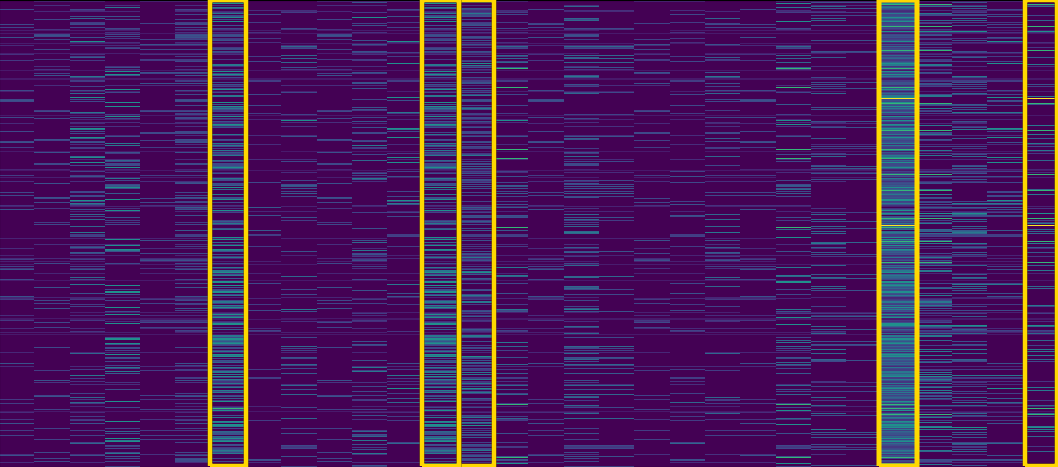
\includegraphics[scale=0.35]{hp_getm_summ_vis}
\caption{\label{fig:hp_summ_getm}}
\end{figure}

Accross all of the Harry Potter GETMS, the major entities are Hermione, Ron, and Harry, which are highlighted by the first 3 yellow box from the left to the right of figure~\ref{fig:hp_summ_getm}, these entities have strong associations with all with almost all terms in the document as well as with terms accross the corpus, for this GETM describing the summary document for Harry Potter and the Philosophers Stone, Hagrid is also a significant Entity. Additional interesting quicks of the model are that the entities  Quirrel and Harry strongly associate to common terms that other entities do not, perhaps suggesting a someform of underlying relationship between those entities.


\clearpage
\subsection{GETM Comparison}



\subsection{GETM Interpretation}
The GETM visualisation could provide an additional utility through which narratives could be analysed. When applying the method to Alice's Adventures in Wonderland, associations between terms and entities produced some interesting results for interpreting narratives latent meanings in narratives.

Considering the novel Alice's Adventures in Wonderland, Figure~\ref{fig:entity_top_terms} highlights the top terms associated with the entity 'Wonderland'. Whilst requiring human interpretation (and some degree of artistic license), the GETM could be interpreted as describing 'Wonderland' as being nothing more than a 'Believed wonderland' and is in reality a 'suppressed misery'. Whilst interpretations such as these are subjective and often personal reflections, it is notable to consider that it was a numerical device that assisted in the task.

\clearpage
\section{Entity Topic-Models}
The use of a GETM was proposed as a means removing an assumption made in literature regarding the relationships which entities have with the topics within a document. It is therefor necessary to evaluate how the adapted approach affects the production of ETMS.

When examining the pairwise scatter matrix for the topics of each entity in the model, you can begin to see some of the differences that the GETM has on the produced ETMs. Figure ~\ref{fig:hp_etm} shows the distributions for the Harry Poter corpus when using a Gaussian Entity Term Matrix configured to use a Gaussian weighting function. There is clearly a spread in structure of Entity Topic Models, though it is acknowledged that interpreting the figure in this form is difficulat, visually identifying any potential any groups of ETMS is not necessarily clear.. The pairwise plots for topics 1, 2, 3, 6, 7, and 8 are shown at a larger scale in figure~\ref{fig:etm_closeup}, from which you can begin to get a sense for some variability in entities and their topical make up. For many of the topic pairs, there is a high density areas, where entities are topically realted to each other, however there is a distict shape to these clouds that could be intereted as distinct groupings. Plots of Entity topics 5 against 1, and 5 against 3, there is an almost triagular shape to the distribution, which may indicate some latent structure amongst the Entity topic models.

Figure ~\ref{fig:hp_summary_etm} visually shows the Entity Topic Models extracted from document summaries, it is clear that they are different to those of the full narratives. Principally, there is a large reduction in the numbers of entities within each document of the corpus, which allows clusters within the collection of Entity Topic Models to be visually identified a little easier. When considering the plotting of Topics 6, and 2, there are three potential clusters , with the most significant being entites strongly represented by only one of the two topics.

It is important to note, that Topics of one set of Entity Topic Models do not directly match up to the Topics of the other set of Topic Models. With the corpora containing different distributions of terms, the term distributions within the topics will also vary greatly. For example, Topic 5 of Figure~\ref{fig:hp_etm} forms similar patterns to Topic 0 of Figure~\ref{fig:hp_summary_etm}. Without numerically evaluating the similarities of each entity topic model, visually comparing is by no means a valid evaluation of consistency between the sets of Entity topic models.

\clearpage
\subsection{Harry Potter Corpus ETMs}

\begin{figure}[h!]
  \centering
  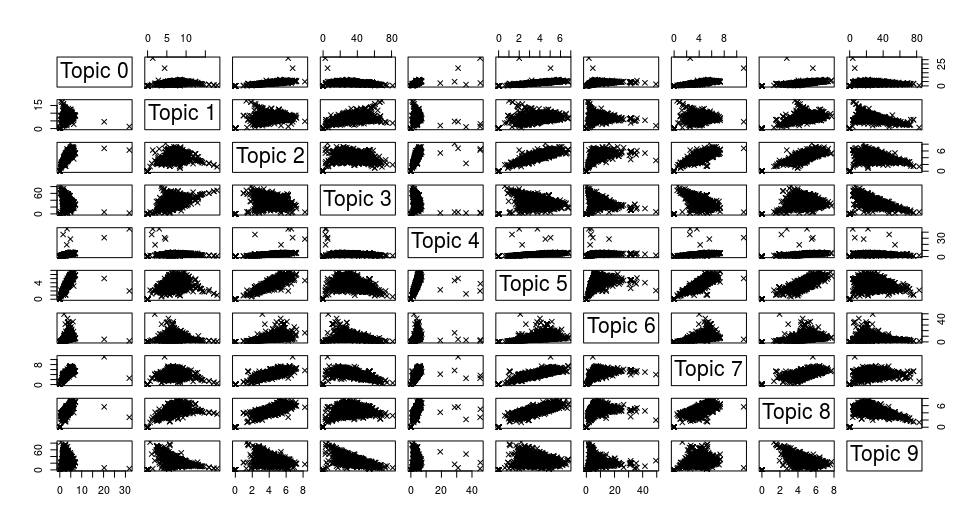
\includegraphics[scale=0.5]{hp_etms}
  \caption{ETM Pairwise Scatter Matrix for Entities in the Harry Potter Novels.\label{fig:hp_etm}}
\end{figure}

\begin{figure}[h!]
  \centering
  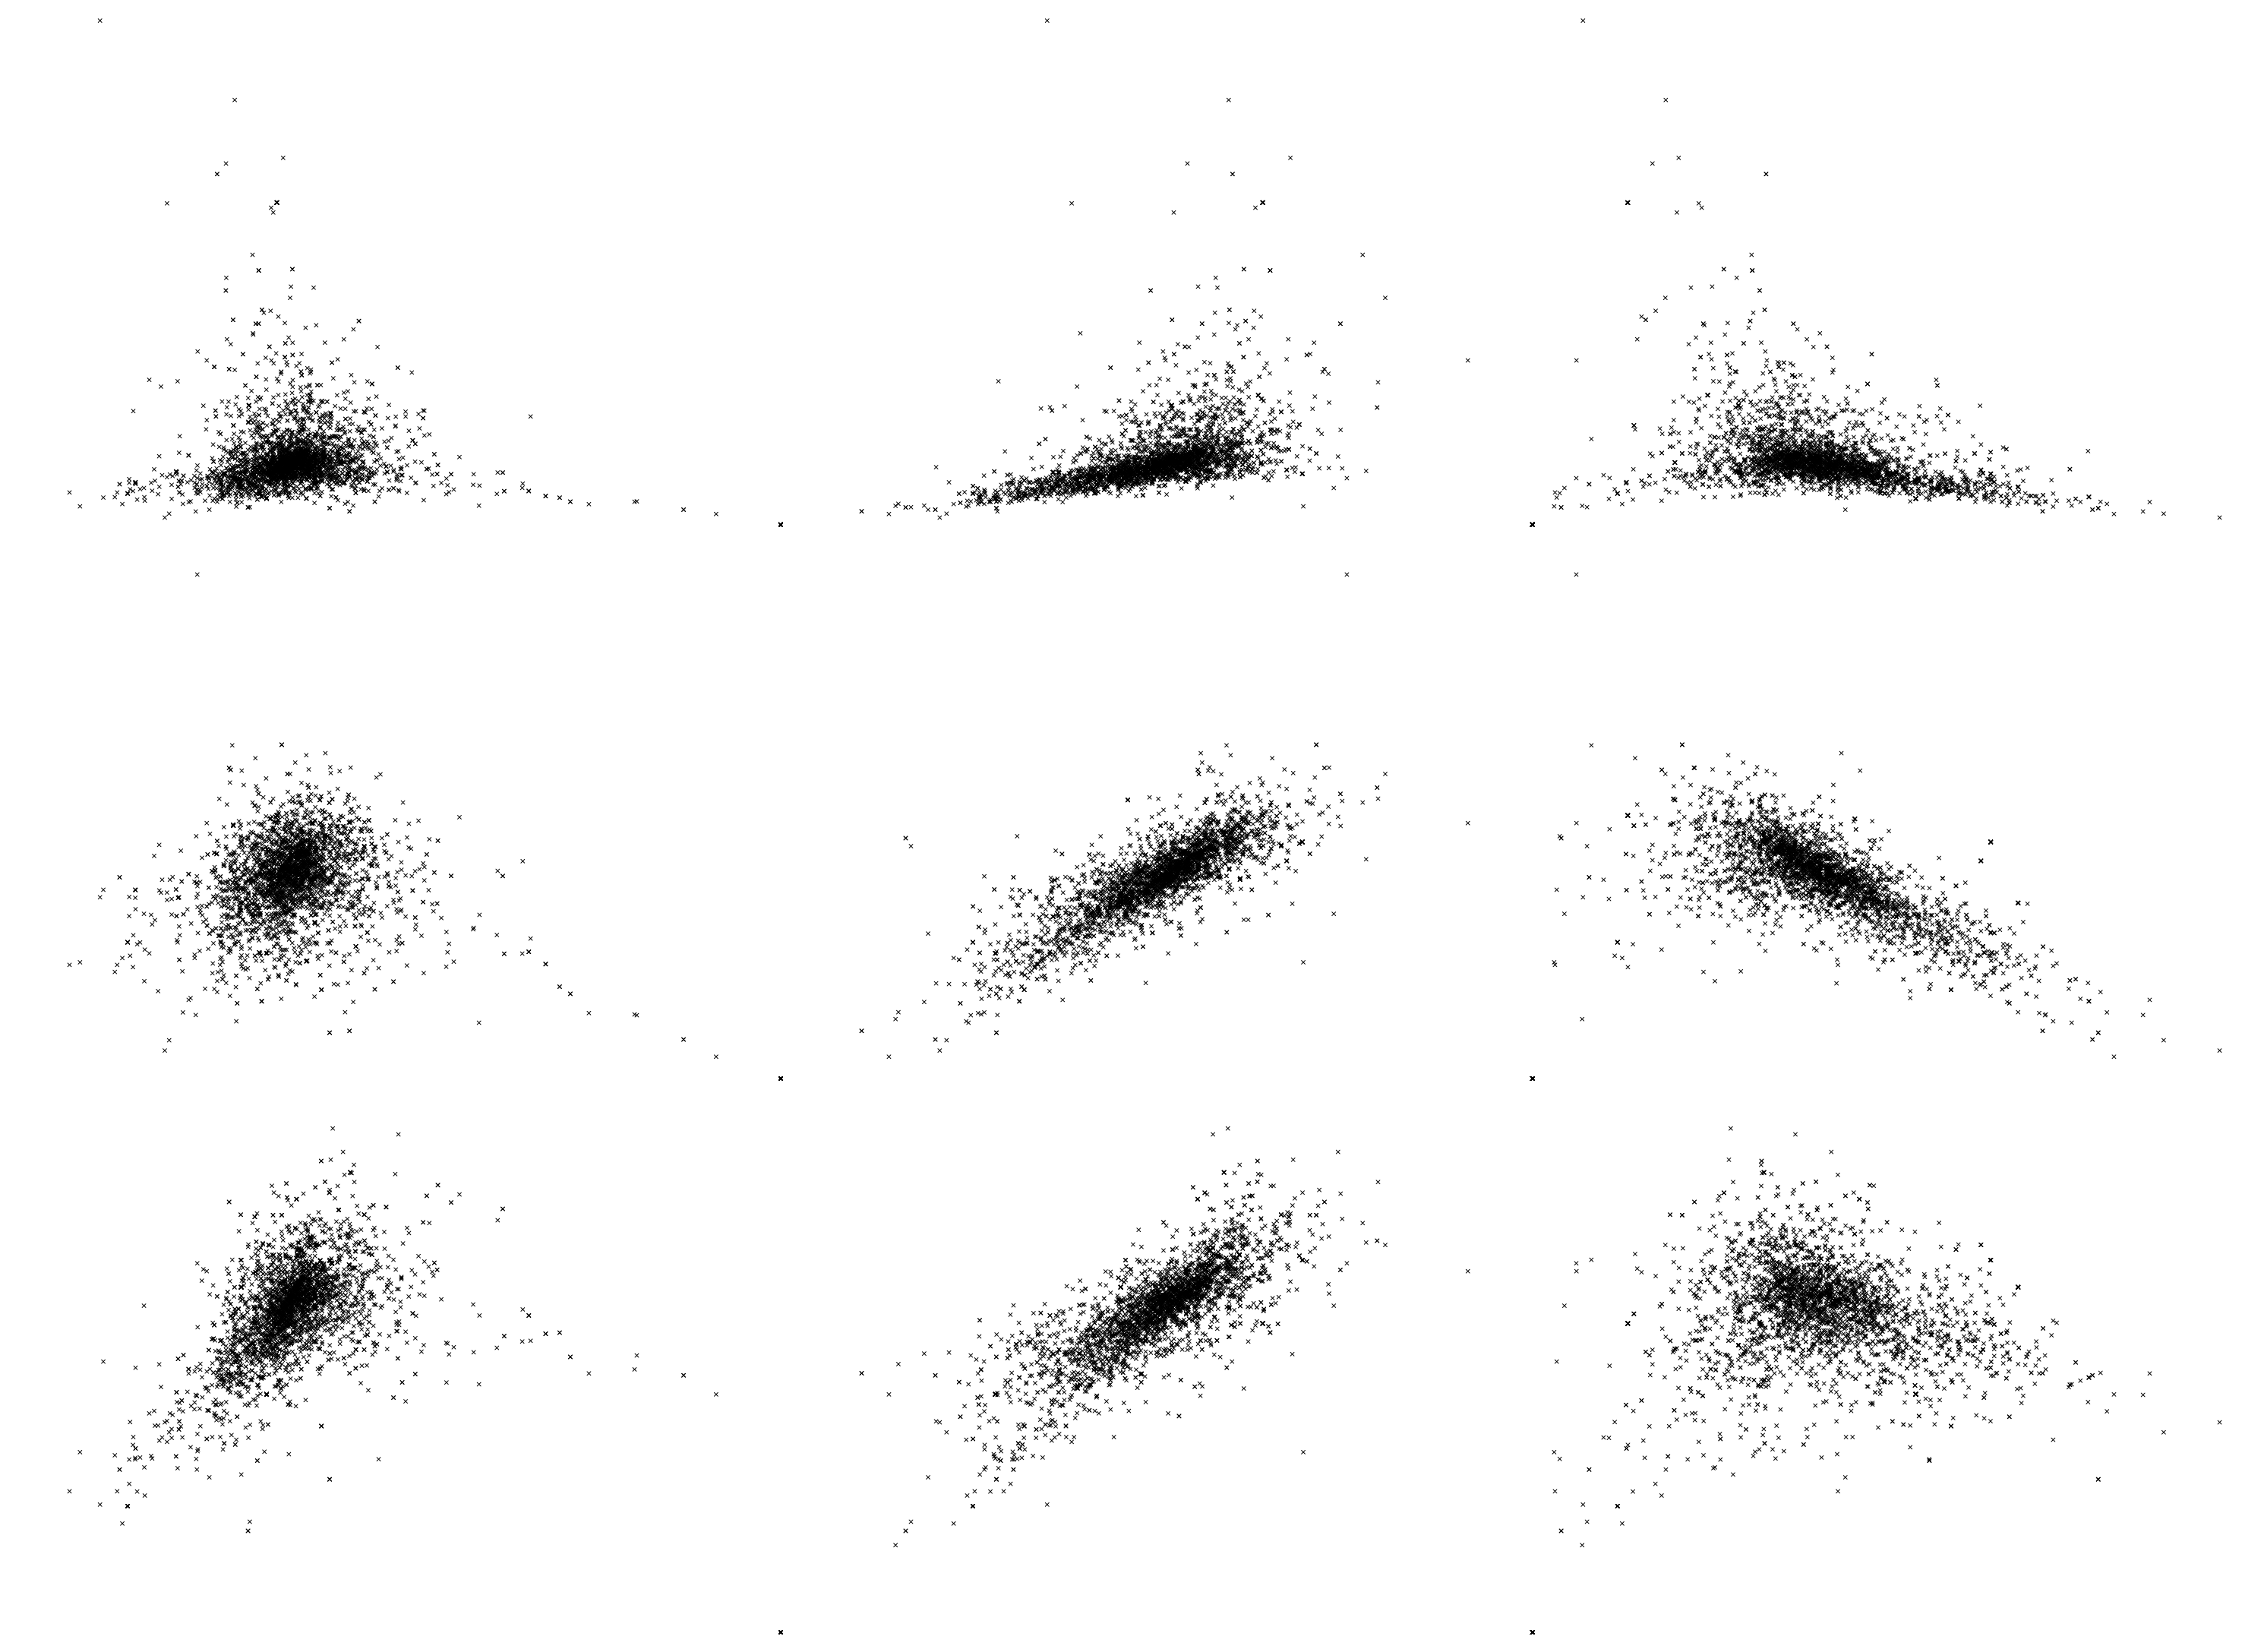
\includegraphics[scale=0.10]{etm_closeup}
  \caption{ETM Pairwise Scatter Matrix Zoomed in on A Selection of Topics of the Harry Potter Novels. \label{fig:etm_closeup}}
\end{figure}


\clearpage
\subsection{Harry Potter Summary Corpus ETMs}

\begin{figure}[h!]
  \centering
  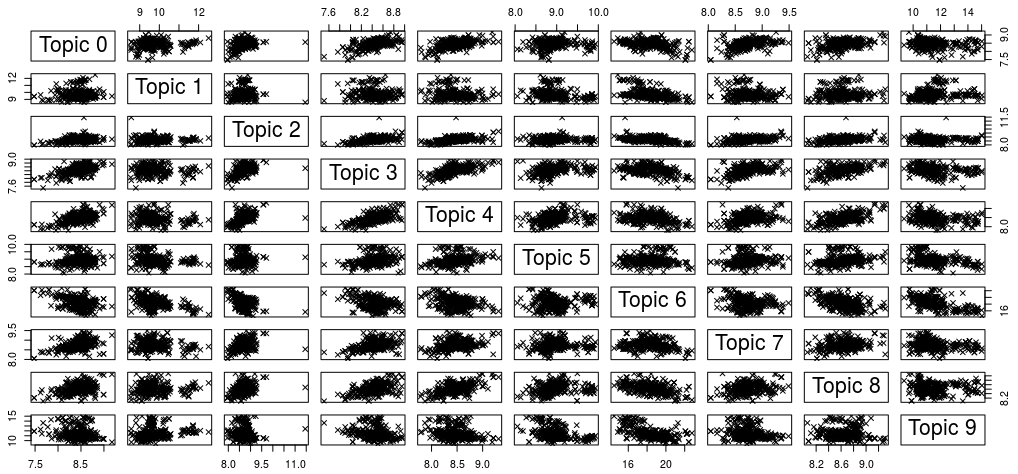
\includegraphics[scale=0.5]{hp_etms_summary}
  \caption{ETM Pairwise Scatter Matrix for Entities in the Harry Potter Novel Summaries.\label{fig:hp_summary_etm}}
\end{figure}

\clearpage
\subsection{ETM Comparison}

\clearpage
\section{Latent Entities}
The evaluation of Latent Entities is a challenging task for two reasons. The first challenge is the lack of labelled data sets which a models performance can be evaluated on, the second difficulty is the subjective nature of the context which the methods have been developed for. Given that narratives and fictional stories are often debated and discussed, with meanings and interpretations varying from individual to individual, it raises the question of whether there ever could be a data set through which Latent Entity Models can be effectively evaluated.

There have been two metrics for Latent Entities that this thesis proposed as a means of evaluating the quality and value of produced models. Consistency is a proposed metric for evaluating the similarity of models trained on different corpora, and is of value for both Latent Entity models, as well as the previously discussed GETM. The second metric is a measure how well an individual can interpret a model which indicates how cohesive a latent entity model is.

The corpus pairings defined in this chapter will form the basis for evaluating the consistency of the models as well as the cohesiveness. 

\clearpage
\subsection{Harry Potter Corpus Latent Entities}
\begin{figure}[h!]
  \centering
  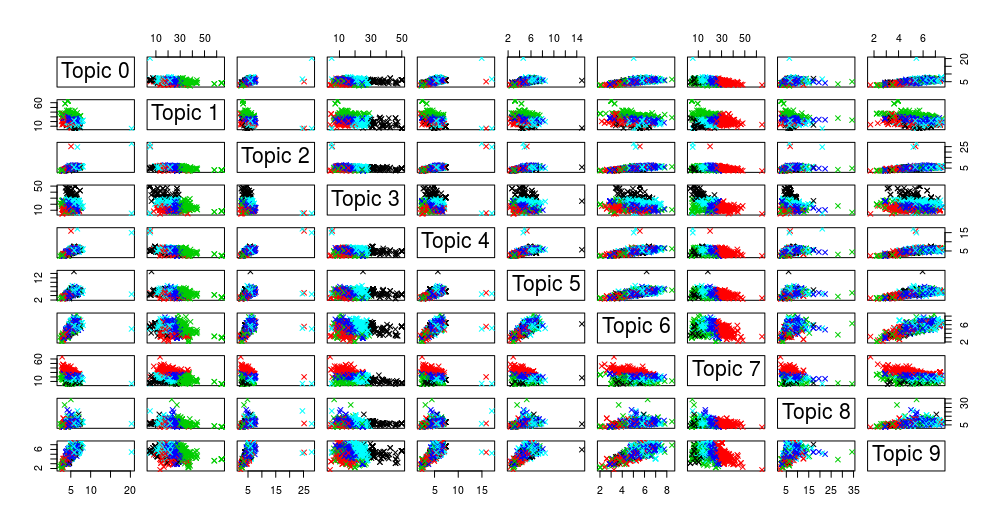
\includegraphics[scale=0.55]{hp_full_latent_entity_scatter}
\caption{\label{fig:hp_le_clusters}}
\end{figure}


\begin{figure}[h!]
  \centering
  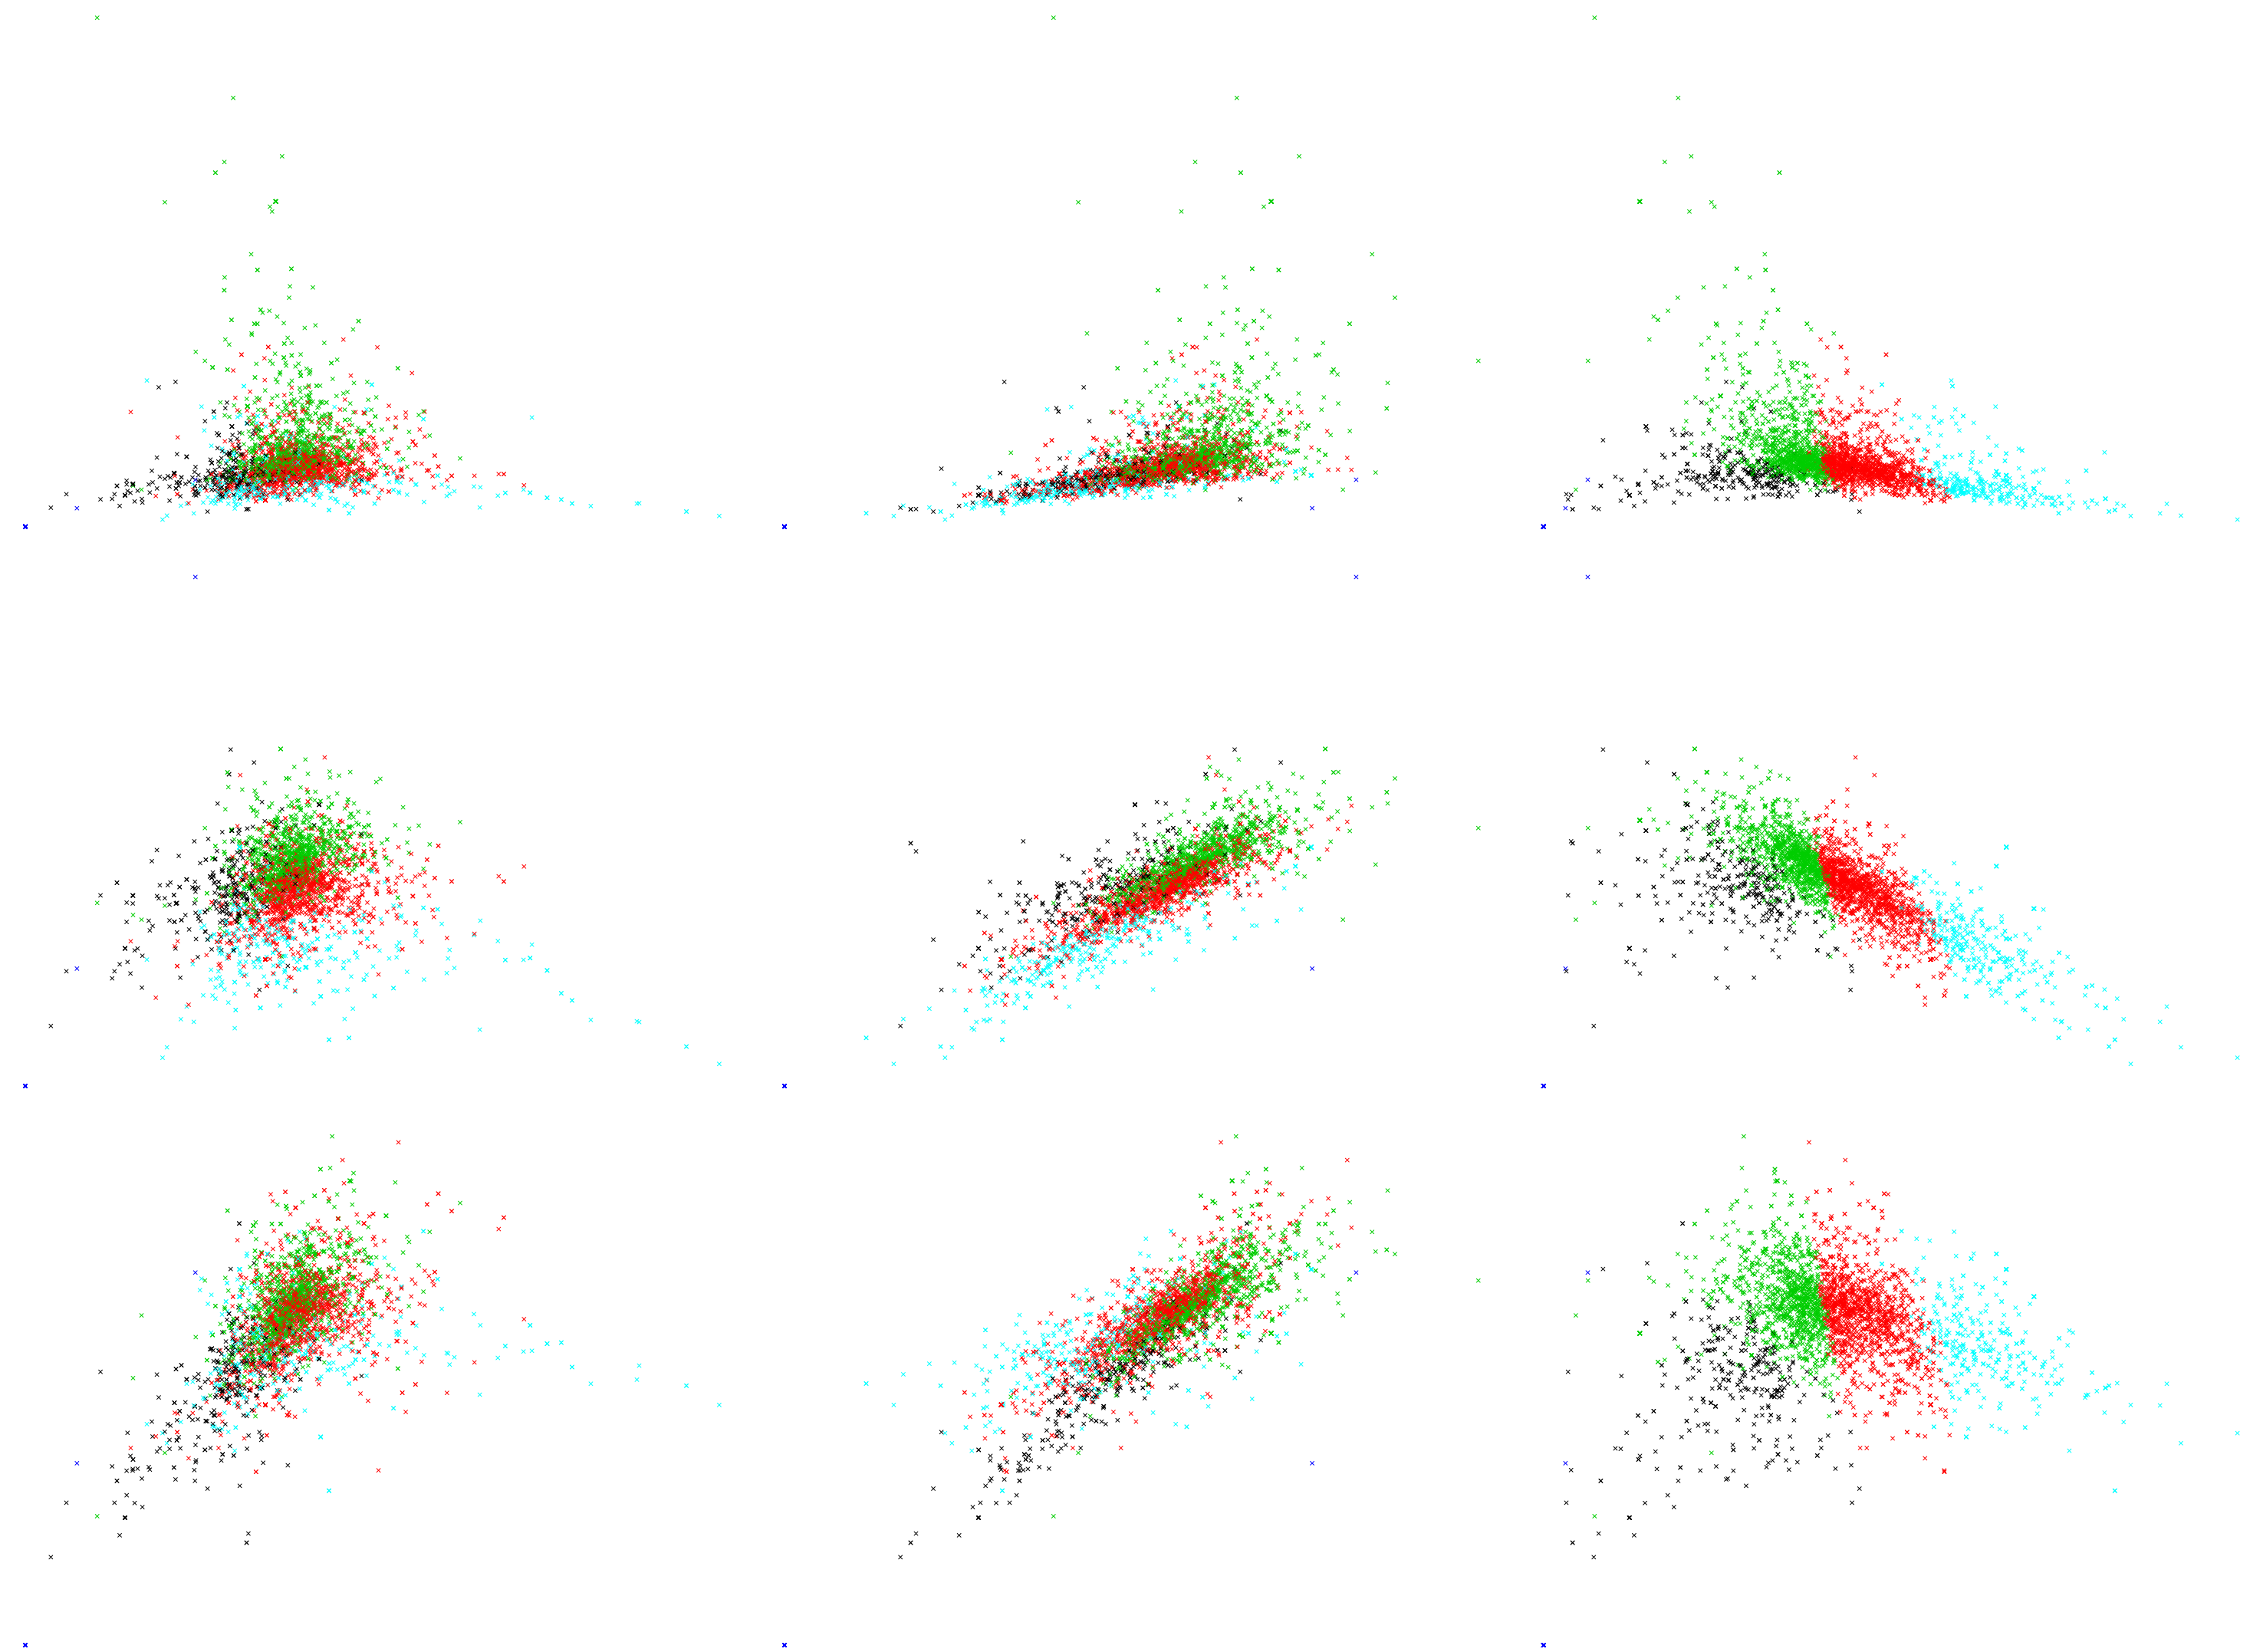
\includegraphics[scale=0.14]{hp_le_cluster_zoom}
\caption{\label{fig:hp_le_cluster_zoom}}
\end{figure}



\clearpage
\subsection{Harry Potter Summary Corpus Latent Entities}



\renewcommand{\baselinestretch}{1.0}\normalsize
\renewcommand{\arraystretch}{1.2}
\begin{table}[h!]
  \centering
  \resizebox{0.32\textwidth}{!}{%
  \begin{tabular}{c | c | c }
    \multicolumn{3}{c}{Latent Entity 0}\\
    Entity    & Distance & Origins\\
    \hline
    hermione  & $0.41$   & Half Blood Prince\\
    snape     & $0.49$   & Half Blood Prince\\
    hogwarts  & $0.61$   & Half Blood Prince\\
    voldemort & $0.65$   & Half Blood Prince\\
    dumbledore& $0.66$   & Half Blood Prince
  \end{tabular}}
  \resizebox{0.32\textwidth}{!}{%
  \begin{tabular}{c | c | c }
    \multicolumn{3}{c}{Latent Entity 1}\\
    Entity    & Distance & Origins\\
    \hline
    sirius  & $0.48$   & Order of the Phoenix \\
    hermione& $0.49$   & Order of the Phoenix \\
    ron     & $0.54$   & Order of the Phoenix \\
    harry   & $0.59$   & Order of the Phoenix \\
    umbridge& $0.60$   & Order of the Phoenix 
  \end{tabular}}
  \resizebox{0.32\textwidth}{!}{%
  \begin{tabular}{c | c | c }
    \multicolumn{3}{c}{Latent Entity 2}\\
    Entity    & Distance & Origins\\
    \hline
    hall      &	$ 0.59 $ & Prisoner of Azkaban \\
    great     &	$ 0.59 $ & Prisoner of Azkaban \\
    hogsmeade &	$ 0.60 $ & Prisoner of Azkaban \\
    scabbers  &	$ 0.66 $ & Prisoner of Azkaban \\
    hagrid    & $ 0.73 $ & Prisoner of Azkaban 
  \end{tabular}}
  \resizebox{0.32\textwidth}{!}{%
\begin{tabular}{c | c | c }
    \multicolumn{3}{c}{Latent Entity 3}\\
    Entity    & Distance & Origins\\
    \hline
    flamel      & $ 0.50 $ & Philosopher's Stone \\
    mcgonagal   & $ 0.67 $ & Philosopher's Stone \\
    dursleys    & $ 0.74 $ & Philosopher's Stone \\
    dumbledore  & $ 0.75 $ & Philosopher's Stone \\
    hermione    & $ 0.76 $ & Philosopher's Stone 
  \end{tabular}}
    \resizebox{0.32\textwidth}{!}{%
  \begin{tabular}{c | c | c }
    \multicolumn{3}{c}{Latent Entity 4}\\
    Entity   & Distance & Origins\\
    \hline
    ron      & $ 0.30 $ & Chamber of Secrets \\
    hermione & $ 0.37 $ & Chamber of Secrets \\
    hogwarts & $ 0.45 $ & Chamber of Secrets \\
    harry    & $ 0.48 $ & Chamber of Secrets \\
    tom      & $ 0.60 $ & Chamber of Secrets  
  \end{tabular}}
  \caption{Entity Topic Models most strongly represented by each Entity Topic Model.\label{tab:hp_le_summs}}
\end{table}

\renewcommand{\baselinestretch}{2.0}\normalsize
\renewcommand{\arraystretch}{1.0}

\clearpage
\subsection{Consistency}
Consistency is evaluated using 3 pairs of copora, the first set of results consider the performance of the model when comparing a corpus of novels to a corpus to summarieis of those novels. 

\clearpage
\subsection{Cohesion and Interpretation}

Prominent Latent Entities that influence the calculation of Latent Entities can be seen in ~\ref{tab:hp_le_summs}, the significance of an entity to the Latent Entity was determined by calculating the euclidean distance between the all Entity Topic Models and Latent Entitie. The most notable aspect of the Latent entities derived from the Harry potter summaries is that the top five for each Latent Entity originate from the same document. There is some degree of variation in the origin document for Entity Topic Models for Entities in the top 10 and top 20. 




\clearpage
\section{Explorer Evaluation}
Evaluating the implemented Explorer web application and associated system requires consideration of the rational behind why the system was required. The quality of the implemented system can be assessed a side from any strengths or weaknesses of the models that the system supports.

With regards to usability of the system, there are two aspects to the system, the command line interface, and the web application interface. The command line interface is simple and requires providing the directory of the corpus files which are to be analysed, there are no other settings for configuration. The limited interface somewhat reduces the flexibility of the analysis pipeline, built within the NLP toolkit is flexibility with regards to some of the hyper parameters within implemented models, including the choice of weighting function, as the number of topics, the number of terms to include within each topic, and the number of latent entities which the system should derive. As a result of excluding these parameters from command line arguments, the pipeline requires manually configuring from within the code base, reducing the accessibility and usability as a whole. 




%
%
% Chapter 6
%
%
\chapter{Conclusion}

\section{Introduction}

\renewcommand{\baselinestretch}{1.0}\normalsize
\bibliographystyle{unsrt}
\bibliography{./biblio}
\end{document}
